\input{preambulos/config}

\begin{document}

\renewcommand{\contentsname}{Contenido}
\renewcommand{\tablename}{\textbf{Tabla}}
\renewcommand{\figurename}{\textbf{Figura}}
\renewcommand{\listtablename}{Lista de tablas}
\renewcommand{\listfigurename}{Lista de figuras}

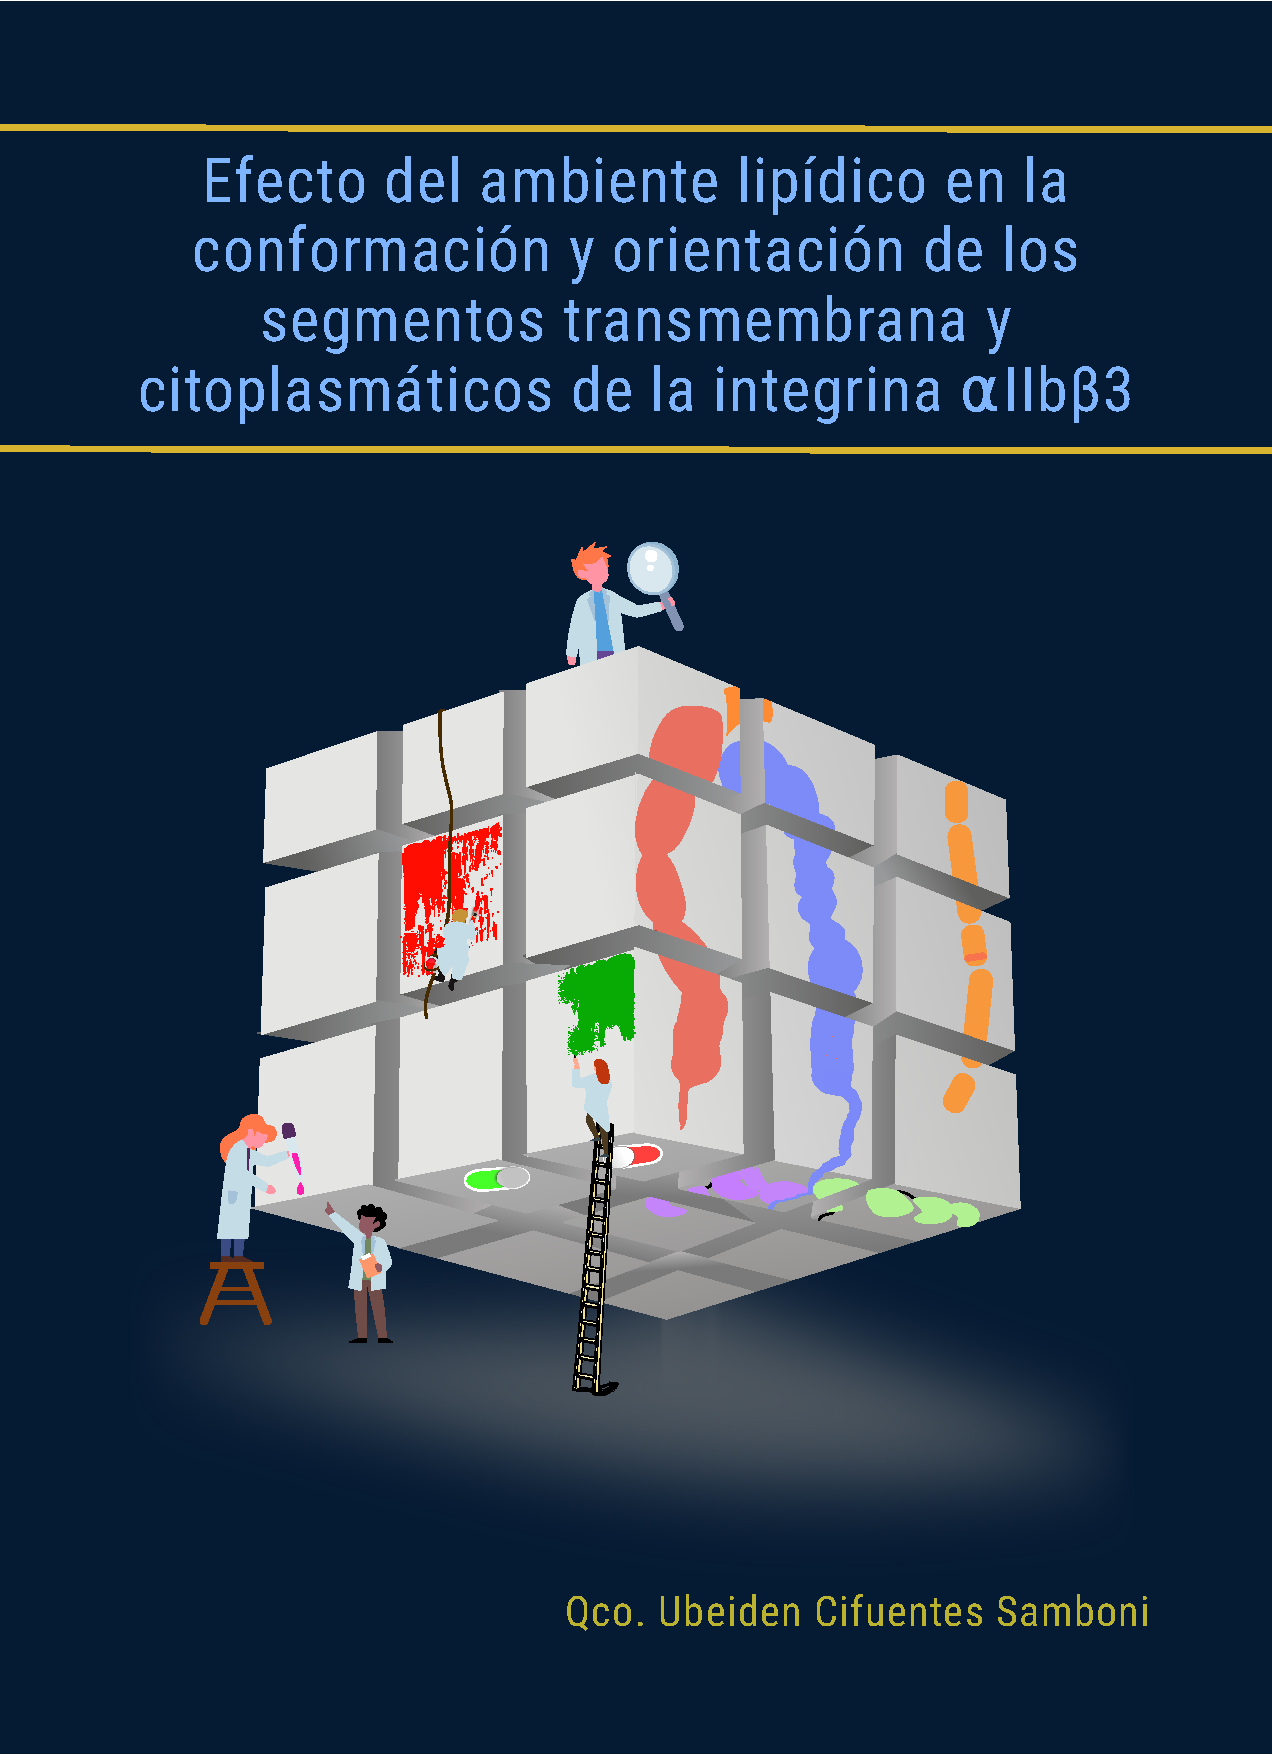
\includepdf[scale=1.03, page=-]{porta_cover/front.pdf}
%\frontmatter
\thispagestyle{empty}
%\chapter*{Agradecimientos}
{\LARGE \textcolor{myblue}{Acerca de la portada}}\\

\begingroup
\setlength{\parindent}{0pt} % Disable indentation within this group

La portada frontal intenta recrear el estado actual del conocimiento sobre las integrinas, combinándolo con un hobby personal: los cubos de Rubik. Las integrinas descubrieron relativamente hace poco tiempo y la información acerca de los mecanismos moleculares y termodinámicos involucrados en la actividad biológica de cada integrina es aún un área en estudio. Incluso, la estructura secundaria y terciaria de ciertos miembros de la gran familia de integrinas no se conoce con exactitud.

La cara derecha del cubo muestra el modelo de la estructura secundaria de las integrinas junto con ciertos ligandos de la matriz extracelular. En la cara inferior se representan algunos ligandos que interactúan con los segmentos citoplasmáticos de las integrinas, además de dos switches, uno de encendido y otro de apagado, que corresponderían al estado activo e inactivo de algunas integrinas. En la cara izquierda, se observa a varios científicos y científicas investigando sobre el tema, para luego plasmar esa información en las aristas, esquinas y centros del cubo. \\\vspace{10cm}


 \tiny {La ilustración tiene un carácter meramente pedagógico y simplificado. No pretende representar con exactitud la realidad de los procesos biológicos de las integrinas.}


\endgroup
\thispagestyle{empty}

%%Escudo de fondo 
\begin{tikzpicture}[remember picture,overlay]
    % Include the image in the background
    \node[anchor=center, opacity=0.1] at (current page.center)
    {\includegraphics[width=0.6\paperwidth]{fig/00_logo/escudo.pdf}};
\end{tikzpicture}


%%Escudo pequeño
\begin{tikzpicture}[remember picture,overlay]
     Include the image in the background
    \node[anchor=north west,, opacity=0.99] at ([shift={(2cm,-3.5cm)}]current page.north west)
    {\includegraphics[width=0.2\paperwidth]{fig/00_logo/escudo.pdf}};
\end{tikzpicture}


\begin{tikzpicture}[remember picture, overlay]
    % Dibujar la línea vertical
    \draw[myblue, line width=3.5pt, opacity=0.85] (3cm,2.2cm) -- (3cm,-18cm);
    
    % Texto alineado a la derecha
    \node[right, text width=10.8cm] at (3.3cm, -8.cm) {
        \thispagestyle{empty}
%       \doublespacing
		\setstretch{2.3}
		\begin{raggedright} 
       \textcolor{myblue}{\Huge\textbf{\!\!\!Efecto del ambiente lipídico en la conformación y orientación de los segmentos transmembrana y citoplasmáticos de la integrina $\alpha$IIb$\beta$3}} \\[3.0cm]
       \end{raggedright} 
       \setstretch{1.3}
        \LARGE\textbf{Qco. Ubeiden Cifuentes Samboni}\\[1.5cm]
        \normalsize Director: Dr. Guillermo Gabriel Montich\\[2.0cm]
        \small Facultad de Ciencias Químicas\\ Departamento Química Biolólogica Ranwel Caputto\\
        Centro de Invistigación de Química Biológica de Córdoba\\
        Universidad Nacional de Córdoba \\[2.0cm]
        \begin{tabular}{@{}llllllll@{}}
          Julio, 2024   & & & & & & & Córdoba, Argentina
        \end{tabular}
    };
\end{tikzpicture}

\setcounter{page}{1}
\pagenumbering{Roman}
\include{porta_cover/portada2}
%\frontmatter
\thispagestyle{empty}
%\chapter*{Agradecimientos}
{\LARGE \textcolor{myblue}{Agradecimientos}}\\

\begingroup
\setlength{\parindent}{0pt} % Disable indentation within this group
% Cómo iniciar esta sección. Son muchas las dudas acerca de cuál es la mejor forma de dar las gracias 

Mi más sincero agradecimiento,\\\vspace{-0.6cm}

A la casa, la que llamamos  \textit{Alma Mater} la Universidad Nacional de Córdoba, particularmente a la Facultad de Ciencias Químicas. Al Centro de Investigaciones en Química Biológica de Córdoba (CIQUIBIC) y el Departamento de Química Biológica Ranwel Caputto (DQBRC) por el lugar de trabajo, los recursos y la formación académica y profesional durante toda mi formación como estudiante de doctorado.\\\vspace{-0.6cm}

Al Consejo Nacional de Investigaciones Científicas y Técnicas (CONICET) y al Fondo para la Investigación Científica y Tecnológica (FONCyT) por el financiamiento como becario doctoral y los espacios de participación científico-académicas. Al Ministerio de Ciencia, Tecnología e Innovación de Colombia por el apoyo económico.\\\vspace{-0.6cm}

A los integrantes de la comisión asesora: Dra. Virginia Miguel, Dr. Ernesto Esteban Ambroggio y Dr. Maximiliano Burgos Paci por las sugerencias y acompañamiento durante todos estos años y por sus aportes en el proceso de escritura de esta tesis. También al evaluador externo, el Dr. Mario Gabriel Del Pópolo quien amablemente aceptó la tarea de leer y evaluar la tesis, además, por sus aportes tan valiosos para la versión final de este documento.\\\vspace{-0.6cm}

A todo el grupo del Dr. Barra (Marilla, Tatiana, Javier, Agustina y el Dr. Barra) donde llegué sin tener la menor idea de cómo hacer un cultivo en placa, me enseñaron las bases de expresión y purificación de proteínas (la primera vez que largué cultivo la mano me temblaba exageradamente pero Agustina siempre me tuvo paciencia, creo). También agradezco a la Dra. Maria Elena Carrizo quien desde mis primeros pasos en la purificación de proteínas me tuvo paciencia y compartió su conocimiento y asesoró en cada momento que acudí a ella.\\\vspace{-0.6cm}

A Daniela y Vanina de FACEMES por los galones (no litros) de medio cultivo que me preparaban para mis purificaciones. Y cómo no agradecer a esas personas que me solucionaron los trámites administrativos: Inés, Alejandra, Magali y Maria Julia. No menos importante, al personal de limpieza y mantenimiento del DQBRC. En general a todo el personal de CIQUIBIC. Seguiré extrañando ``la pescadeada'' cada primero de mayo.\\\vspace{-0.6cm}

A la Dra. Vanessa Galassi por la orientación en los primeros pasos en el mundo de las simulaciones de dinámica molecular durante mi visita en Mendoza, sobre todo, por llevarme a escalar. A su linda familia Gastón, Iñaki y ``la Ile''. También agradecer a todos los miembros del grupo del Dr. Mario G. Del Pópolo del ICB-UNCUYO por compartir las charlas en los almuerzos.\\\vspace{-0.6cm}

A los doctores Martin Ulmschneider y Chris Lorenz por la gran oportunidad para visitar sus grupos de investigación en el King's College London. Aquí aprovecho para agradecer a Raquel, brillante joven científica siempre predispuesta a ayudar. Gracias por los momentos compartidos y por aventurarse a visitarnos en Argentina. Usted e Iván ahora son unos amigos ``al otro lado del charco''.\\\vspace{-0.6cm}

A las chicas súper poderosas: Laura, Jesica y Anabela quienes terminaron primero que yo pero la amistad que generamos aún perdura. También agradezco al ahora Dr. Christian que ya hacía parte del selecto grupo de las poderosas. Gracias por las charlas deprimentes (``...y sí'' dicen ustedes), motivadoras y académicas durante los almuerzos y por las caminatas saludables.\\\vspace{-0.6cm}

Continuando con las charlas en los almuerzos un agradecimiento a: el grupo de la reina  Yohana y sus súbditos (Genero, Pedro y Franco). También a Luz, Verónica (la más ruidosa de toooodo el CIQUI, alias ``10 L''), Ana, Agustina, Rocio, Flor y Maxi (``el capo de los dibujos''). Y si hablamos de comida, gracias a Manuel, Alain, Ricardo y Román por esas juntadas prepandémicas.\\\vspace{-0.6cm}

A la Sociedad Argentina de Biofísica y en especial a la comunidad de los Jóvenes Biofísicos - YIB por los espacios de discusión científico-académica y por la red de contactos con personas maravillosas de diversas provincias del país y de otros países de Latino América.\\\vspace{-0.6cm}

A las investigadoras e investigadores del área de Biofísica: las  doctoras Laura, Natalia y Soledad, y los doctores Gerardo, Rafael y Ernesto por su gentileza para compartir todo lo de su laboratorio y por la asesorías académicas. Por supuesto gracias a los compañeros y compañeras de biofísica por las comidas en los seminarios y charlas de pasillo: Beny, Nahuel, Ignacio, Ezequiel, Leandro, Cande, Dr. Matías, Iván, Juan (``el putas de aguadas''), Jessica, Nocelli, Dario y Nacho (``de la comunidad del anillo''). Hablando de charlas, le agradezco al Dr. Ariel Goldraij por las charlas de historia de Latino América y por las sugerencias de películas colombianas para este colombiano. Un especial agradecimiento a Maca y al Dr. Agustín por la amistad, mi admiración para ustedes. Gracias al doctor Guillermo, mi director por darme la oportunidad de ser su becario doctoral, por siempre mantener la calma y serenidad. Gracias doctor por compartir su conocimiento sobre proteínas y por los momentos de discusión, en lo no académico por siempre ofrecer su ayuda cada vez que lo necesitaba y por las charlas de ciclismo por supuesto. \\\vspace{-0.6cm}

A Carla y su familia: ``el Ale'', Franca y Salvador por permitirme llegar a su casa y prácticamente ser un miembro más de la familia. Y hablando de familia, Maia, Xul, Sole y Mauri mi familia argentina, en especial Sole por siempre estar ahí para escuchar, abrazar, sonreír y hablar (\textexclamdown sobre todo!). Eres ``amor puro'' y fui afortunado de conocerte, muchas gracias Sole.\\\vspace{-0.6cm}

A las amistades colombianas, Lucía \& Fabián, Eliana \& Didier, Melina \& Felipe, Einy y Maria José gracias por compartir fechas de navidad, cumpleaños y asados. Gracias a mi primer mentor, el profe Alberto quien influyó en gran medida en mi decisión para aventurarme a hacer un doctorado. Como no agradecer a mi entrenador de alto rendimiento, el profe Ruben Dario, gracias por la formación deportiva y sobre todo por sus enseñanzas humanas. Un especial agradecimiento a Stefanía por su amistad tan hermosa y por siempre brindar una sonrisa a cambio de un cafecito.\\\vspace{-0.6cm}

A las personas más importantes en mi vida, \textbf{mi familia} primas, primos, tías y tíos, en especial a mis tíos en La Tebaida Quindío y particularmente a mi tío Enrique. A mi madre Lucy y mi padre Laurentino con quienes estaré eternamente agradecido por toda la educación familiar, el cuidado y el amor que me dan. A mi hermano Fabián y hermana Ligia por aceptarme desde mi llega a su casa y siempre estar ahí para mí. Por otra parte, más que un agradecimiento una dedicatoria a mi familia biológica, mi madre Marina, hermanas y hermanos. Y como no agradecer a mi \textit{fiancée} Amoy, gracias a ti la pandemia fue más llevadera, gracias por siempre estar al otro lado de la pantalla dispuesta a escucharme y por el amarme incondicionalmente (también por la paciencia \textexclamdown claro!).\\\vspace{-0.6cm}

Por último, agradecer al pueblo argentino. Por financiar a través de sus impuestos mi educación de posgrado.\\\vspace{1cm}

\begin{flushright}
Ubeiden Cifuentes Samboni
\end{flushright}
\endgroup
\tableofcontents


\frontmatter
\newpage
%\frontmatter
\thispagestyle{empty}
\section*{Resumen}

Las integrinas son proteínas integrales de membranas. Son grandes receptores de superficie celular heterodiméricos ($\alpha$\!$\beta$) que desempeñan un papel clave en la formación de complejos de adhesión a la matriz extracelular y están involucrados en varias vías de transducción de señales. La integrina $\alpha$IIb$\beta$3 está presente en plaquetas y es el principal modulador del proceso de agregación de plaquetas. En el estado desactivado, los segmentos transmembrana de la integrina $\alpha$IIb y de $\beta$3 forman un heterodímero con orientación relativa definida. La disociación del heterodímero y la consecuente activación del receptor esta mediada por la unión de ligandos citoplasmáticos a segmento intracelular de $\beta$3. Las interacciones que establecen los segmentos transmembrana en el heterodímero son determinantes para la funcionalidad del receptor. En está tesis empleamos monocapas de Langmuir como sistema de membrana modelo, y simulaciones de dinámica molecular en bicapas lipídicas para estudiar la función del ambiente lipídico en la conformación y orientación de los segmentos transmembrana e intracelular de la integrina $\alpha$IIb$\beta$3.

De estos estudios surgieron una serie de ideas novedosas, entre ellas: (i) los péptidos presentan una orientación vertical respecto al plano de las monocapas de Langmuir; (ii) el análisis de polaridad sugiere que el segmento intracelular está en contacto con la subfase acuosa y el segmento transmembrana queda expuesto hacia el aire; (iii) la presencia de los péptidos modifica las propiedades reológicas de la membrana como la tensión superficial, elasticidad lateral y módulo de compresibilidad; (iv) se observó que el segmento de $\alpha$IIb interacciona preferentemente con lípidos en estado líquido expandido (POPC o la mezcla POPC-POPG) que un lípido en estado líquido condensado (DPPC); (v) en general, el ambiente lipídico modula las interacciones y la orientación entre los segmentos transmembrana del heterodímero. 

Los resultados experimentales y bioinformáticos presentados aquí demuestran la importancia de comprender las propiedades del entorno en el que se encuentran las proteínas de membrana y el impacto que la naturaleza del ambiente lipídico tiene sobre sus conformaciones y funcionalidad.


\newpage
\thispagestyle{empty}
\section*{Abstract}

Integrins are examples of integral membrane proteins. They are large heterodimeric cell surface receptors ($\alpha$-$\beta$) that play a key role in forming adhesion complexes with the extracellular matrix and are involved in several signal transduction pathways. Integrin $\alpha$IIb$\beta$3 is found in platelets and is the primary modulator of platelet aggregation. In its inactive state, the transmembrane segments of integrin $\alpha$IIb and $\beta$3 form a heterodimer with a specific relative orientation. The dissociation of this heterodimer, leading to receptor activation, is triggered by the binding of cytoplasmic ligands to the intracellular segment of $\beta$3. The interactions established by the transmembrane segments in the heterodimer are crucial for the functionality of the receptor. In this thesis, we use Langmuir monolayers as a model membrane system, along with molecular dynamics simulations in lipid bilayers, to study the role of the lipid environment in the conformation and orientation of the transmembrane and intracellular segments of the integrin $\alpha$IIb$\beta$3.

From these studies, a series of novel ideas emerged, including: (i) the peptides have a vertical orientation with respect to the plane of the Langmuir monolayers; (ii) Polarity analysis suggests the intracellular segment is in contact with the aqueous subphase and the transmembrane segment is exposed to the air; (iii) the presence of the peptides alters the rheological properties of the membrane, such as surface tension, lateral elasticity, and compressibility modulus; (iv) it was observed that lipids such as POPC and PCPG preferentially interact with the $\alpha$IIb peptide; and (v) in general, the lipid environment modulates the interactions and orientation between the transmembrane segments of the heterodimer..

The experimental and bioinformatics results presented here demonstrate the importance of understanding the properties of the environment in which membrane proteins are found, as well as the impact that the nature of the lipid environment has on their conformations and functionality.

\addcontentsline{toc}{chapter}{Resumen} 
\clearpage

\newpage
\include{preambulos/abreviaturas}
\addcontentsline{toc}{chapter}{Lista de abreviaturas} 
\clearpage

\listoffigures
\addcontentsline{toc}{chapter}{Lista de figuras} % para que aparezca en el indice de 
\clearpage
\listoftables
\addcontentsline{toc}{chapter}{Lista de tablas} % para que aparezca en el indice de contenidos
\clearpage

\setcounter{page}{1}
\pagenumbering{arabic}

\mainmatter
\include{chap/cap1}
\chapter{Metodología}\label{chap:metod}

\section{Metodología experimental}

\subsection{Plásmidos, reactivos, equipos y materiales}
La secuencia de los segmentos \ac{tm}-\ac{ic} de los péptidos $\alpha$IIb y $\beta$3 fueron donados por el laborario del Dr. Jun Qin \citep{Yang2009}. Cada plásmido fue clonado en la cepa de bacteria \ac{ecoli} DH5$\alpha$. Los plásmidos clonados fueron purificados usando un kit de purificación de ADN ``Wizard Plus SV Miniprep'' (Promega, Madison, WI, USA). El \ac{iptg} fue adquirido en Gentbiotech. Las  columnas  de Sefarosa Ni HisTrap HP  5 mL y de desalado PD-10 fueron adquiridas en GE Healthcare (Cat. 71-5027-68 Cat. 17085101, respectivamente). Para el \ac{hplc} se usó en equipo Agilent Technologies 1260 Infinity con detector de arreglo de diodos y longitud de onda múltiple (DAD VL), equipado con software ChemStation/Open LAB; columna Ultisil XB-C4, 5 $\mu$m, 300 Å, 4.6x250 mm, cat.00216-33043 (Welch SKU. H00216-33043, USA). Las membranas de celulosa (Dialysis Tubing, Benzoylated, poro de 2000 MWCO) fueron adquiridas en SIGMA. La concentración de proteína fue determina en espectrofotómetro Varian 2300, (Palo Alto, CA, USA). Las \ac{sds} y disoluciones amortiguadoras fueron preparadas usando agua grado Milli-Q tipo 1. Los análisis de \ac{em} se realizaron en un espectrómetro de masas ESI-Qq-TOF (Bruker). 
Los lípidos \ac{popc}, \ac{popg}, \ac{dppc}, fueron adquiridos en Avanti Polar, USA; el  \ac{chcl3}, \ac{acn} y \ac{meoh} grado \ac{hplc} en la firma Merck, Alemania.

\subsection{Extracción y clonación de plásmidos}
%%Para redactar ver parte se soporte del paper Qin & Jun
%%%https://www.sciencedirect.com/science/article/pii/S0168165622003042?via%3Dihub
%%% diagrama del plasmido https://sci-hub.se/10.1080/10409230490514008
Ambos plásmidos pMAL-c2 (New England Biolabs, Inc., Beverly, MA) fueron replicados por separado en la cepa \emph{E. coli} DH5$\alpha$ (ver \textbf{protocolo} \ref{Protocolo Plasmido}). Este vector contenía la secuencia que codifica cada péptido y la \ac{mbp} para facilitar un primer paso de purificación que llamaremos ``proteína fusión''. Entre el N-terminal de la \ac{mbp} y el C-terminal de cada péptido hay una secuencia de hexahistidina o His$_{6}$-\emph{tag} y sitio de corte para la proteasa del \ac{tev} que permiten separar cada secuencia de interés en dos pasos de purificación (\textbf{figura} \ref{fig:plasmido}). Además, posee la secuencia \emph{amp$^r$} que permite seleccionar bacterias que incorporen el plásmido con ampicilina. Todos los medios y material utilizado, así como el agua Milli-Q fueron esterilizados en autoclave por 30 minutos a 1.2 atm de presión y 120\textdegree C.

%%%%%%%%%%%%%%%%%%%%% Fig plasmido %%%%%%%%%%%%%%%%%%%%%%%%
\begin{figure}[h] % supposedly places it here ...
    \centering
	\includegraphics[width=0.69\linewidth]{fig/01_expe/pmal_c2.pdf}
	\caption[Esquema del plásmido pMAL-c2 - $\alpha$IIb/$\beta$3]{Esquema plásmido pMAL-c2 - $\alpha$IIb/$\beta$3. Figura adaptada de Vector Database por \href{https://www.addgene.org/}{addgene.org} (2023). Extraído de \href{https://www.addgene.org/vector-database/3506/}{https://www.addgene.org/vector-database/3506/}.
        \index{plasmido}}
    \label{fig:plasmido}
\end{figure}
%%%%%%%%%%%%%%%%%%%%% Fin %%%%%%%%%%%%%%%%%%%%%%%%


\subsection{Expresión y purificación de la proteína fusión}\label{sec:expre_akta}

Una vez propagado el plásmido de cada péptido en bacterias \emph{E. coli} DH5-$\alpha$ se expresó la proteína fusión en una cepa de bacterias \emph{E. coli} BL21(DE3), ver \textbf{protocolo} \ref{Protocolo_Fusion}. Posteriormente se lisaron las bacterias y se purificó la proteína por afinidad a níquel en \ac{fplc}.
Se cuantificó cada proteína fusión por espectrofotometría \ac{uv} teniendo en cuenta los coeficientes de absortividad molar, {\Large{$\varepsilon$}} a 280 nm: {\Large{$\varepsilon$}}$_{\alpha \text{IIb}}$ = 85830 M$^{\text{--1}}$ cm$^{\text{--1}}$, {\Large{$\varepsilon$}}$_{\beta\text{3}}$ = 83310 M$^{\text{--1}}$ cm$^{\text{--1}}$; valores obtenidos de \url{https://web.expasy.org/protparam/}. El rendimiento de cada \textbf{proteína fusión} fue de 10 y 15 mg/L cultivo para $\alpha$IIb y $\beta$3,  respectivamente.

Por otra parte, también se expresó y purificó la proteasa \ac{tev} en nuestro laboratorio. El plásmido de la proteasa TEV (donado por el laboratorio del Dr. Ernesto Ambroggio) se inoculó en la cepa \emph{E. coli} BL21(DE3) y se purificó por afinidad a níquel.

\subsection{Clivaje y diálisis}

La proteína fusión fue incubada con la proteasa \ac{tev} y se dejó a 30\textdegree C por $\Xapprox$ 48 horas. Se centrifugó y  se recuperó el sobrenadante y se dializó en membranas de celulosa contra agua con agitación constante a 4\textdegree C. El contenido de las membranas se centrifugó en tubos eppendorf a 13000 \ac{rpm} por 10 minutos, \textbf{precipitando el péptido transmembrana} (en el sobrenadante se separó \ac{mbp}, \ac{tev} y proteína fusión sin cortar). El pellet se resuspendió en \ac{acn}:H$_{2}$O 40\%:60\% (vol/vol) con \ac{tfa}, consultar \hyperref[Protocolo_TEV]{\textbf{protocolo} \ref*{Protocolo_TEV}} para más detalle.

\subsection{Repurificación por \ac{hplc}}

%%%%%%%%%%%%%%%%%%%%% Tabla pequeña %%%%%%%%%%%%%%%%%%%%%%%%
\begin{wraptable}{r}{3.5cm}
\vspace{-0.63cm} %%%Posiciona a una altura en la hoja
\centering
    \caption{\\Gradiente HPLC.}\label{tab:hplc_gradiente}
    \begin{tabular}[t]{ccc}%%%
     \toprule  % <-- Toprule here
      {Min}  & {A\%} & {B\%}\\
      \hline
        0       &  60    & 40  \\
        7       &  58    & 42 \\
        8       &  54    & 46  \\
        10      &  48    & 52 \\
        15      &  44    & 56  \\
        20      &  40    & 60 \\
        25      &  36    & 64  \\
        30      &  32    & 68 \\
        35      &  28    & 72  \\
    \textbf{40} & \textbf{24}    & \textbf{76} \\
        45      &  15    & 85  \\
        50      &  5     & 95 \\
        55      &  0     & 100  \\
      \bottomrule % <-- Bottomrule here
    \end{tabular}
    \vspace{-6cm} %%%Posiciona texto debajo tabla
    \end{wraptable} 
%%%%%%%%%%%%%%%%%%%%% Fin %%%%%%%%%%%%%%%%%%%%%%%%

Se realizaron múltiples cromatografías inyectando 1.0 mL de muestra bajo las siguientes condiciones cromatográficas:

\begin{tabularx}{\textwidth}{@{}p{0.20\textwidth} p{0.85\textwidth}@{}}
Fase móvil A: & 40\% H$_{2}$O(+0.1\% \ac{tfa}) \\
Flujo:              & 1.0 mL/min        \\ 
Temperatura:        & 40\textdegree C              \\
Presión máxima:     & 210 bar           \\
Detector UV:        & 280 nm            \\
Inyección:          & 1.0 mL (manual)     \\
Fase móvil B:   & 100\% \ac{acn}(+0.1\% \ac{tfa}) \\
\end{tabularx}


Se colectaron todas fracciones de la cromatografía según el gradiente de la \textbf{tabla} \ref{tab:hplc_gradiente} y se verificó la pureza por geles \ac{sds} y por \ac{em}.  Los péptidos purificados fueron solubilizados en \ac{acn}:H$_2$O 67\%/33\% (vol/vol); la concentración se determinó por absorbancia \ac{uv} teniendo en cuenta los {\Large{$\varepsilon$}} a 280 nm para cada péptido: {\Large{$\varepsilon$}}$_{\alpha \text{IIb}}$ = 16500 M$^{\text{--1}}$cm$^{\text{--1}}$, {\Large{$\varepsilon$}}$_{\beta \text{3}}$ = 13980 M$^{\text{--1}}$cm$^{\text{--1}}$. La remoción de \ac{tfa} y verificación de estructura secundaria de los péptidos se realizó por espectroscopía \ac{ftir}-\ac{atr}. El rendimiento final fue de 400 $\mu$g/L cultivo para $\alpha$IIb y 600 $\mu$g/L para $\beta$3. Se fraccionaron y almacenaron a -20\textdegree C para su posterior uso (ver \hyperref[Protocolo_HPLC]{\textbf{protocolo} \ref*{Protocolo_HPLC}}).

\subsection{Electroforesis en gel y \ac{em}}

%%https://core.ac.uk/download/pdf/71054185.pdf
La pureza de ambos péptidos fue confirmada por geles SDS-PAGE y \ac{em}. Al tratarse de péptidos altamente hidrofóbicos se prepararon geles de poliacrilamida al 18\% en condiciones desnaturalizantes con \ac{sds}, junto con las muestras se sembró un marcador de peso molecular como referencia. La electroforesis se corrieron a 125 V y 4\textdegree C.

Se preparó una solución 100 $\mu$M de péptido en \ac{acn}:H$_2$O 67\%/33\% (vol/vol) + 0.1\% ácido fórmico y se inyectó en el espectrómetro de masas. El espectro fue adquirido en modo ion positivo desde 250 a 30000 m/z, con flujo de inyección de $\mu$L/min. El procesamiento de los datos se realizó en el software Data Analysis de Bruker. Se promediaron dos cromatogramas, se procesó por deconvolución de la carga después de haber sustraído la línea base y se realizó un suavizado para obtener un cromatograma de alta resolución relación masa-carga m/z. Alternativamente los datos fueron post-procesados usando el Algoritmo de Máxima Entropía para obtener un espectro de masa neutra. Para ambos péptidos se obtuvo la masa esperada para los monómeros.

\subsection{Experimentos de monocapas de Langmuir}

Los experimentos de monocapas de Langmuir fueron realizados a temperatura ambiente (20\textdegree C). Todos los stock de soluciones de lípidos fueron preparadas en \ac{chcl3}:\ac{meoh} 2:1 (vol/vol). Las monocapas se realizaron en una unidad de control de Monofilmeter (con Film Lift, Mayer Feintechnique, Alemania). La presión superficial ($\pi$) se midió usando el método de Wilhelmy con una placa Platinized-Pt y el potencial superficial ($\Delta$V) se detectó mediante el uso de una placa ionizante de americio ($^{241}$Am) y un electrodo de calomelanos conectados a un voltímetro. Los datos fueron registrados de forma continua y simultánea con un registrador X-YY de doble canal. El área superficial total de la cuba de Teflón fue de 80 cm$^2$ con capacidad de $\Xapprox$ 75 mL para la subfase (PBS 20 mM, NaCl 100 mM a pH 7.4). Para los péptidos puros se evaporó el solvente ACN:H$_2$O con flujo de nitrógeno (N$_{2 \text{(g)}}$) y se realizaron al menos 3 lavados con CHCl$_3$:MeOH 2:1 (vol/vol). La monocapa se formó sembrando 0.5 nmoles de péptido en solución de CHCl$_3$:MeOH  en la subfase usando una jeringa Hamilton. Tanto para la isoterma del lípido puro como para las mezclas con péptidos se procedió de forma similar y se esperó por 8 minutos antes de empezar la compresión para dar tiempo a la evaporación del solvente y posteriormente se empezó a comprimir a razón fija de $\Xapprox$ 5.3 \AA $^{\text{2}}$ molécula$^{\text{--1}}$ s$^{\text{--1}}$. Antes de sembrar las muestras se realizaron los respectivos controles, para la superficie limpia y los disolventes de las muestras, en donde no se observó actividad superficial de los disolventes. Cada experimento se realizó por triplicado de forma independiente y se prepararon soluciones frescas de cada lípido cerca al momento de utilizarse.

Se realizaron ciclos de compresión-expansión, inicialmente las barreras se fijaron en 60 cm$^2$, se inició la compresión hasta llegar a los $\Xapprox$ 13 cm$^2$ y se expandió hasta los $\Xapprox$ 60 cm$^2$ y así se repitió tres veces para cada muestra.

\section{Metodología computacional}

\subsection{Preparación de los sistemas}

Las simulaciones grano grueso se realizaron usando el campo de fuerza Martini 2 \citep{DeJong2013}, las coordenadas los dominios transmembrana-citoplasmático de la integrina $\alpha$IIb$\beta$3,  fueron tomadas de la base de datos proteínas ``\textit{Protein Data Bank}'' identificados con el código PDB 2KNC \citep{Yang2009}. Se usó el servidor CHARMM-GUI \citep{Wu2014} para insertar el heterodímero $\alpha$IIb$\beta$3 en una bicapa, el cual implementa los programas martinize.py \citep{DeJong2013} e INSANE (\textit{INSert membrANE}) para producir la estructura Martini de los lípidos y proteína, respectivamente \citep{Wassenaar2015}. Además, se hidrató el sistema con agua tipo PW \citep{Yesylevskyy2010}, finalmente se agregaron partículas sodio y cloro hasta una concentración 0.15 M de NaCl. Se aplicó una red elástica aplicada (ElNeDyn) \citep{Periole2009} sobre las partículas C$_\alpha$ de cada péptido usando un radio de corte de 7 \AA con una constante de 10 kJ mol$^{\text{--1}}$ \AA $^{2}$, el heterodímero $\alpha$IIb$\beta$3  fue insertado en 4 membranas de diferente composición cada una compuesta de 250 lípidos por hemicapa (POPC, POPG, POPC:POPG 70:30 (PCPG), DPPC). El sistema se minimizó por 1000 pasos usando el método \textit{steepest descent} \citep{Haug1976}, posteriormente se equilibró en condiciones \textit{NVT}: número de partículas (N), volumen (V) y temperatura (T) constantes  por 5 ns aplicando restricciones de posiciones para los $C_\alpha$ en las regiones con $\alpha$ hélice. Finalmente, las simulaciones  se realizaron con el software de libre distribución GROMACS (\textit{GROningen MAchine for Chemical Simulations}) \citep{Lindahl2019}. Se usó el termostato de Berendsen \citep{Berendsen1984} y el barostato Parrinello-Rahman \citep{Parrinello1981} para mantener la temperatura a 320 K (excepto el sistema con DPPC que se simuló a 340 K) y la presión a 1 atmósfera con acoplamiento semi-isotrópico con una compresibilidad de 4.5 x 10$^{\text{--5}}$ bar$^{\text{--1}}$. Las interacciones eletrostáticas de largo alcance fueron incorporadas a través del método de partículas de  Ewald con un radio de corte de 1 nm. El mismo radio de corte se aplicó para las interacciones Lennard-Jones.
Los dinámicas se produjeron con los recursos de cómputo del \ac{sncad} usando los clúster Mendieta, Serafín (CCAD-UNC, \href{http://ccad.unc.edu.ar}{http://ccad.unc.edu.ar}) y el clúster Create del King’s College London (\href{https://docs.er.kcl.ac.uk/CREATE/access/}{https://docs.er.kcl.ac.uk/CREATE/access/}). 

\subsubsection{Análisis de datos}

El procesamiento de los datos experimentales y de la dinámicas se realizaron con código Python haciendo uso de las librerías  Numpy, Pandas \citep{Harris2020, McKinney2010}. Todos los gráficos fueron generados con las librería Matplotlib y Seaborn \citep{Hunter2007, Waskom2021}. El análisis de trayectorias se realizó con el paquete GROMACS y la librería MDAnalisys \citep{Jo2011}. La visualización de las trayectorias se realizó con el software NGLView \citep{Nguyen2018}.

\include{chap/cap3}
\chapter{Interacción lípido-péptido en monocapas de Langmuir}\label{chap:mono}


\section{Monocapas de péptidos puros}\label{mono_pept_puros}

\begin{figure}[b!]
\vspace{0.5cm} 
    \centering
	\includegraphics[width=0.85\linewidth]{fig/01_expe/orienta_pept2.png}
	\caption[Esquema de posible orientación de hélice $\alpha$ en el plano de una monocapa.]{Esquema de posible orientación de hélice $\alpha$ en el plano de una monocapa. A) Orientación perpendicular-\textit{i)} o  paralela-\textit{ii)} al plano de la monocapa. B) Vista lateral y superior del segmento TM $\alpha$IIb donde se muestra la longitud y el radio. \textit{L}$_{1}$ es la distancia entre los carbonos alfa del TRP$^{967}$ y la PHE$^{993}$, \textit{L}$_{2}$ distancia entre los carbonos alfa de la GLY$^{955}$ y el GLU$^{1008}$.}
        \index{orientacion}
    \label{fig:orientTM}
\end{figure} 

Antes de analizar los resultados de moncapas de Langmuir de los péptidos puros, surge la pregunta \textquestiondown cuál es la posible orientación de los péptidos en la interfase agua-aire? En las proteínas nativas, ambos péptidos tienen estructura hélice $\alpha$. Si consideramos a un péptido transmembrana como un cilindro (\textbf{figura} ~\ref{fig:orientTM}B), podemos inferir acerca de su orientación a partir de las medidas de área molecular en capas monomoleculares. Un área molecular experimental similar al área de la base del cilindro indicaría un arreglo de péptidos orientados perpendicularmente a la interfase y altamente compactados como se representa en la \textbf{figura} ~\ref{fig:orientTM}A-\textit{i}. Con los datos de los estructura secundaria de los péptidos (PBD 2KNC) \citep{Yang2009} se calculó el radio de los segmentos TM de $\alpha$IIb y $\beta$3. Usando la librería MDAnalysis \citep{Jo2011} se implementó un algoritmo para determinar el eje principal de cada segmento TM. El radio se calculó como la distancia promedio entre el eje principal y el átomo  \textit{X} (\textit{X}: C, N, O, S) de cada residuo más distante al eje. Se determinó un radio promedio de 6.1 Å y 6.6 Å para $\alpha$IIb y $\beta$3 respectivamente. Con estos valores de radios se esperarían áreas moleculares de  $\Xapprox$ 117 Å\textsuperscript{2} para $\alpha$IIb y $\Xapprox$ 137 Å\textsuperscript{2} para $\beta$3. Por lo tanto, cerca de la presión de colapso ó en un punto de inflexión en la curva presión-área de los péptidos puros se esperaría observar un área molecular con éstos valores, indicando que su orientación es perpendicular al plano de la monocapa. Valores mayores del área corresponderían a otras orientaciones no perpendiculares o en estados conformacionales expandidos, desordenados y no correspondientes con hélice $\alpha$. En el caso que los péptidos se orienten horizontalmente y considerando que los segmentos TM que tienen estructura hélice $\alpha$ se conserva, las área moleculares esperadas son de 1555 Å\textsuperscript{2} para $\alpha$IIb (r=$\frac{L_1}{2}$) y 3366 Å\textsuperscript{2} para $\beta$3 (r=$\frac{65.5 \, \text{Å}}{2}$).

\begin{figure}[b!] % supposedly places it here ...
\vspace{0.5cm}
    \centering
	\includegraphics[width=0.5\linewidth]{fig/01_expe/mono/isoPept.png}
	\caption[Isotermas de compresión en la interfase agua/aire de los péptidos puros.]{Isotermas de compresión en la interfase agua/aire de los péptidos puros.}
        \index{isoPept}
    \label{fig:isoPept}
\end{figure}
%%%%%%%%%%%%%%%%%%%%% Fin %%%%%%%%%%%%%%%%%%%%%%%%

Ambos péptidos presentan actividad superficial en monocapas de Langmuir (\textbf{figura}~\ref{fig:isoPept}). Forman monocapas estables que pueden ser comprimidas en al menos dos ciclos de compresión-descompresión sin perder material por partición a la subfase. La siembra de 0.5 nmoles no produjo un aumento de presión significativamente diferente de cero y corresponde a un área de $\Xapprox 2500$ Å\textsuperscript{2}/molécula. Estos valores de área molecular indican que los péptidos tienden a organizarse paralelamente al plano de la monocapa cuando la compresión lateral es poca o nula. A 5 mN/m, los péptidos se han compactado y el área molecular es de  $\Xapprox 1300$ Å\textsuperscript{2} para ambos péptidos. A una presión de 35 mN/m las áreas moleculares fueron $\Xapprox 587$ \textpm \,25 Å\textsuperscript{2} y $\Xapprox 488$ \textpm \,20 Å\textsuperscript{2} para $\alpha$IIb y $\beta$3 respectivamente. Estos valores de área molecular indican que los péptidos tienen un radio aparente de 13.7 Å para $\alpha$IIb y 11.7 Å para $\beta$3. Valores que son cerca de dos veces el calculado. Por lo tanto, éstos valores de área indicarían que los péptidos tienden a orientarse verticalmente (más adelante se discute con mayor detalle). Comparando estos valores de radio experimentales con otros péptidos reportados, varios autores coinciden con un valor de de 5.0 Å para una hélice $\alpha$ \citep{Barlow1988, Kato2015,Ionov2000,Weder2003} el cual daría un área de 78.5 Å\textsuperscript{2}. Para la aurina 2.3 se reportó un radio de 10 Å, valor que correspondería un área molecular de 314.6 Å\textsuperscript{2} \citep{Mura2013}. Valor que se aproxima al observado para los péptidos $\alpha$IIb y $\beta$3.

Otra pregunta que surge es, \textquestiondown el extremo \textit{N-terminal} está expuesto al aire y el extremo \textit{C-terminal} interactúa con la subfase, o es al revés? El no colapso de la monocapa estaría dado por las posibles fluctuaciones de la región que no tiene estructura secundaria definida (segmento \ac{ic}), por tanto a presiones bajas estas regiones son las que se localizan preferentemente en la subfase mientras que las  hélice $\alpha$, región hidrofóbica, se orienta hacia el aire. A medida que se comprime la monocapa, las colas forman ``loops'' que aumentan de tamaño y pueden oscilar a medida que se compacta y por lo tanto no se llega a una presión de colapso (ver \textbf{figura} \ref{fig:mono_pept}, flechas \textcolor{blue}{\faLongArrowRight}), un análisis similar fue reportado para la albumina sérica humana \citep{Toimil2012}. A una presión 35 mN/m el péptido $\alpha$IIb presentó un área molecular mayor al esperado teóricamente (117 Å\textsuperscript{2}), este valor se calculó teniendo en cuenta sólo la región con estructura secundaria hélice $\alpha$, de igual forma con $\beta$3.

\begin{figure}[H] 
    \centering
	\includegraphics[width=0.99\linewidth]{fig/01_expe/mono_pept.png}
	\caption{Modelo de reorganización de los péptidos en monocapas de Langmuir y fluctuación de estructura secundaria en segmento intracelular para los péptidos $\alpha$IIb y  $\beta$3.}
        \index{mono_pept}
    \label{fig:mono_pept}
\end{figure}

Helmholtz propone que la diferencia de potencial de superficie en una monocapa está dado por \citep{Helmholtz1902},

\begin{equation}
    \label{ecu:potencial}
    \Delta V =  \frac{12 \Pi \mu_\perp}{A}
\end{equation}

donde $\Delta V$ es el potencial de superficie (mV) medido entre el seno de la solución acuosa y la fase gaseosa (aire), \textit{A} el área molecular (Å\textsuperscript{2}), $\Pi$ es una constante  y $\mu_\perp$ es el momento dipolar total de superficie. El $\Delta V$, medido en una monocapa tiene tres contribuciones: i) los dipolos ordenados de las moléculas adsorbidas, ii) los dipolos de las moléculas de agua ordenadas en la zona de la superficie, iii) el dipolo generado por la doble capa iónica de Gouy-Chapman en caso que las moléculas adsorbidas tengan cargas netas \citep{Brockman1994,Electronics1994}. Se observó que aún cuando la presión de superficie es indistinguible de cero, el $\Delta V$ es significativamente grande y alcanza valores de entre 200 y 150 mV para $\alpha$IIb y $\beta$3 respectivamente (\textbf{figura} \ref{fig:muDeltaV}A).
%%%$\mu_\perp$ = $\mu_1$ + $\mu_2$ + $\mu_3$, $\mu_1$ es la contribución de las moléculas de agua orientadas al rededor de las caras hidrofílicas de la proteína, $\mu_2$ y $\mu_3$ contribuciones hidrofílica e hidrofóbica de la proteína que esta en contacto con la superficie 
En los dos péptidos el $\mu_\perp$ inicia con valores de $\Xapprox 8.5$ D en $\alpha$IIb y $\Xapprox 12.5$ D en $\beta$3 (\textbf{figura} ~\ref{fig:muDeltaV}B) y a medida que se comprime lateralmente va disminuyendo hasta alcanzar los $\Xapprox 4.3$ D al valor mínimo de área molecular, esta tendencia abre la posibilidad a realizar el siguiente planteamiento de reorganización: inicialmente los péptidos se encuentran con una superficie de contacto mayor expuesta al agua y por lo tanto, hay alta densidad de carga que contribuye al $\mu_\perp$  (\textbf{figura} \ref{fig:mono_pept}A-B-C), sin embargo al compactarse lateralmente, los péptidos tienen a orientarse verticalmente, exponiendo menos residuos a la superficie de la monocapa, disminuyendo la densidad de carga, finalmente se llega a un estado donde están lo suficientemente  compactados de manera que todo lo que tiene estructura hélice $\alpha$ queda expuesto al aire y la única parte que contribuye al $\Delta$V y/o $\mu_\perp$ es la región que fluctúa de estructura y que tiene mayor carácter polar; un planteamiento similar realizó Maget \citep{Maget-Dana1999}.


\begin{figure}[H] % supposedly places it here ...
    \centering
	\includegraphics[width=0.55\linewidth]{fig/01_expe/mono/muDeltaV.png}
	\caption[Potencial de superficie y momento dipolar perpendicular de los péptidos puros en monocapas.]{A) Potencial de superficie y B) momento dipolar perpendicular de los péptidos puros en monocapas.}
        \index{muDeltaV}
    \label{fig:muDeltaV}
\end{figure}
%%%%%%%%%%%%%%%%%%%%% Fin %%%%%%%%%%%%%%%%%%%%%%%%

Para tener una mejor idea de lo planteado anteriormente acerca de cómo se orientan los péptidos en la monocapa de Langmuir, se realizó un análisis de la hidrofobicidad promedio por residuo <H> \, del momento hidrofóbico <$\mu_H$> \,y de la carga de cada péptido (ver \textbf{tabla} ~\ref{tab:mu_hidrofo}). En los dos péptidos, el domino \ac{tm} presenta mayor <H> \, respecto a los segmentos \ac{ec} e \ac{ic}, principalmente dado por la cantidad de residuos hidrofóbicos (\textbf{figura} ~\ref{fig:mu_hidrofo}, resaltados en amarillo \begin{tikzpicture}
  \node[draw, circle, fill=yellow, line width=0.5pt, inner sep=1pt, scale=0.6, font=\color{yellow}] {\faCircle}; \end{tikzpicture}). El <H> \, del segmento \ac{ec} es más grande (0.693\textgreater\!\textgreater -0.091) que el segmento \ac{ic} del péptido $\alpha$IIb, además, el domino \ac{ic} presenta cuatro cargas negativas comparadas a una carga positiva del segmento \ac{ec}. El péptido $\beta$3 tiene 25 residuos más que $\alpha$IIb en el segmento \ac{ic} (\textbf{figura} ~\ref{fig:mu_hidrofo}, ``55-79''), éstos últimos residuos que aportan un caracter hidrofóbico aunque sigue siendo menor comparado al segmento \ac{ec} (0.163\textless\!\textless 0.360), además, hay una carga positiva. Por tanto en los dos péptidos, es más probable que el segmento \ac{ic} interactúe con la fase acuosa, permitiendo así sugerir que los péptidos se orientan con el \textit{del N-terminal} expuesto al aire y el \textit{C-terminal} en contacto con la subfase (\textbf{figura} ~\ref{fig:orientTM}B). Los parámetros de <H> \,y <$\mu_H$> \,fueron calculados según las ecuaciones \ref{ecu:H} y \ref{ecu:muH},

\begin{equation}\label{ecu:H}
   <\!H\!> =  \frac{1}{N} \mathlarger{\Sigma}_{n=1}^NH_n
\end{equation}

donde \textit{N} es el número de residuos en la secuencia, \textit{H$_{n}$} es la hidrofobicidad del residuo \textit{n}. Los valores de hidrofobicidad para cada residuo se pueden encontrar en literatura \citep{Eisenberg1982}. El promedio del momento hidrofóbico <$\mu_H$> \, se calculó según:
%%%ecuación esta en la pagina online https://heliquest.ipmc.cnrs.fr/HelpProcedure.htm#heading2
\begin{equation}\label{ecu:muH}
<\!\mu_{H}\!> =  \frac{1}{N} \left(\left(\mathlarger{\Sigma}_{n=1}^{N}H_n \sin \text{(}\delta n\text{)} \right)^{2}+\left(\mathlarger{\Sigma}_{n=1}^{N} H_n \cos\text{(}\delta n\text{)}\right)^{2}\right)^{\frac{1}{2}}
\end{equation}

%%%%Tabla resumen de H_mu%%%%
\begin{table}[H]
\vspace{-0.5cm} 
\centering
\begin{threeparttable}
\centering
\caption{Resumen de hidrofobicidad y carga para los segmentos \ac{ec}, \ac{tm} e \ac{ic} de péptidos $\alpha$IIb y  $\beta$3.}\label{tab:mu_hidrofo}
\begin{tabular}{@{}llccl@{}}
\toprule
Péptido     & N\textdegree \,Residuo             & <H>      	& <$\mu_H$> 	& z  \\ \midrule
$\alpha$IIb & \multirow{2}{*}{1-11 \; (EC) }  & 0.185  	& 0.025 		& 1- \\
$\beta$3    &                        & 0.360  	& 0.031		& 0  \vspace{3mm} \\
$\alpha$IIb & \multirow{2}{*}{12-36 \;(TM)} & 1.182  	& 0.005 		& 1+ \\
$\beta$3    &                        & 1.183  	& 0.005 		& 1+ \vspace{3mm} \\
$\alpha$IIb & \multirow{2}{*}{37-54 \;(IC)} & -0.091 	& 0.015 		& 4- \\
$\beta$3    &                        & -0.091 	& 0.011 		& 0  \vspace{3mm} \\
$\beta$3    & 55-79 \;(IC)                  & 0.163  	& 0.010 		& 1+ \\ \bottomrule
\scriptsize{\ac{ec}: \acl{ec}} & \scriptsize{\ac{tm}: \acl{tm}} & \scriptsize{\ac{ic}: \acl{ic}}
\end{tabular}
\end{threeparttable}
\end{table}
%%%%%Fin tabla%%%%%

donde $\delta$ es el ángulo de separación de las cadenas laterales a lo largo de la cadena principal, con $\delta$=100\textdegree \,para una hélice $\alpha$ \citep{Eisenberg1982a}. Un valor alto del <$\mu_H$>\,sugiere que la secuencia de proteína puede adoptar una estructura hélice $\alpha$ anfifílica perpendicular a su eje, es decir, <$\mu_H$> \, es una medida de la anfifilicidad de una hélice $\alpha$. Para comparar las magnitudes de los <$\mu_H$> fue necesario trabajar con los valores normalizados por el número de residuos, <$\mu_H$>\,= $\mu_H$/\textit{N}. La región con menor <$\mu_H$> \,es el domino \ac{tm} y la de mayor <$\mu_H$> \,el segmento \ac{ec} (ver \textbf{figura} ~\ref{fig:mu_hidrofo}).
%%%%%%%%%%%%%%%%%%%%% Figura %%%%%%%%%%%%%%%%%%%%%%%%
\begin{figure}[H] % supposedly places it here ...
    \centering
	\includegraphics[width=0.6\linewidth]{fig/01_expe/secuencias_alfa_beta.png}
	\caption[Proyección circular de la hélice para las secuencias de los segmentos TM-IC de $\alpha$IIb y  $\beta$3.]{Proyección circular de la hélice para las secuencias de los segmentos TM-IC de $\alpha$IIb y $\beta$3. La fecha (\textrightarrow) en el centro indica la magnitud y la dirección del momento hidrofóbico <$\mu_H$>. La proyección se realizó con el software HeliQuest  (\url{https://heliquest.ipmc.cnrs.fr/cgi-bin/ComputParams.py}).}
        \index{mu_hidrofo}
    \label{fig:mu_hidrofo}
\end{figure}
%%%%%%%%%%%%%%%%%%%%% Fin %%%%%%%%%%%%%%%%%%%%%%%%

Es importante destacar que la evaluación de la actividad superficial comprende la integración de múltiples factores contribuyentes, entre ellos la anfipaticidad, el tamaño molecular, la flexibilidad estructural, la carga neta y las interacciones intramoleculares. Esta complejidad inherente en la composición y el comportamiento de las moléculas subraya las dificultades en la interpretación del potencial de superficie. Además, es relevante reconocer que, dadas estas variadas influencias, los resultados experimentales relativos a esta propiedad suelen exhibir una considerable variabilidad, manifestándose en una dispersión significativa en comparación con los valores teóricos anticipados. Esta observación resalta la necesidad de un enfoque meticuloso y detallado en la interpretación de los datos experimentales, considerando la gama de variables que pueden afectar las mediciones del potencial de superficie.

\section{Monocapas de Langmuir para mezclas lípido-péptido}\label{sect:mono_mezclas}

Se realizaron isotermas de compresión de lípido puro (\ac{popc}, PCPG, \ac{dppc}) y mezclas lípido-péptido ($\alpha$IIb ó $\beta$3) en concentraciones crecientes de péptido desde 0.0\% a 7.0\% por mol. En la \textbf{figura} ~\ref{fig:area_pi_all}, panel superior se muestran las mezclas de lípido-$\alpha$IIb y en el inferior las mezclas lípido-$\beta$3. En todos los experimentos se realizaron 3 ciclos de compresión-expansión para evaluar la estabilidad del film lípido-péptido. Para la mezcla  \ac{popc}/$\alpha$IIb se observó que en todas las concentraciones de péptido se produjo un corrimiento a áreas mayores respecto al lípido puro, más notable con el incremento de la concentración de péptido. En PCPG/$\alpha$IIb se observó que la mezcla tiende a compactarse o por lo menos a estar más cerca de la isoterma de la mezcla pura PCPG. La isoterma de compresión de DPPC puro presentó un comportamiento típico con una pretransición de la fase \ac{le} a \ac{lc} cerca de los 6 mN/m. Se observaron dos efectos como consecuencia de la presencia de los péptidos: una expansión que es ligeramente mayor a la esperada en una mezcla ideal y la pérdida notoria de la transición LE-LC que es altamente cooperativa. Estos efectos se ha observado en otros péptidos \citep{Saleem2008, Nakahara2011}.
Respecto a las mezclas de lípido/$\beta$3, presentaron comportamientos similares a lo observado con el péptido $\alpha$IIb. En la mezcla con PCPG/$\beta$3 el corrimiento a áreas menores es más marcado en concentraciones de 2.0\% y 3.5\% (\textcolor{falured}{\rotatebox{90}{\faPlay}}), incluso a 2.0\% casi no se diferencia de la isoterma de la mezcla PCPG pura.
Comparando un poco más en detalle el efecto de los dos péptidos, en las monocapas de \ac{popc}, a 5.0\% (\textcolor{goldenpoppy}{\faCircle}) de $\alpha$IIb, la isoterma se desplaza a áreas menores comparado a las concentraciones más bajas que iba aumentando pero luego a 7.0\% (\textcolor{deepmagenta}{$\pentagonblack$}) se recupera dicha tendencia, mientras que en presencia de $\beta$3 sucede el mismo efecto pero a 2.0\% y luego se produce el corrimiento a áreas mayores. Para la mezcla binaria de lípidos PCPG, a bajas concentraciones de péptido (2.0\% y 3.5\%) ya se ve un efecto de compactación, siendo más notorio en presencia de $\beta$3. En las isotermas de \ac{dppc}, se observa un corrimiento a áreas mayores al incrementar la concentración de péptido, esto pasa con ambos péptidos, sin embargo, en presencia de $\beta$3 esa tendencia sigue hasta 5.0\% porque luego a 7.0\% baja a corrimientos similares al 2.0\% de $\beta$3.

%%%%%%%%%%%%%%%%%%%%%Fig. Isotermas de compresión %%%%%%%%%%%%%%%%%%%%%
\begin{figure}[t] % supposedly places it here ...
    \centering
	\includegraphics[width=0.99\linewidth]{fig/01_expe/mono/area_pi_allFinal.png}
\caption[Isotermas de compresión (\boldmath{$\pi$}--A) para mezclas lípido-péptido]{Isotermas de compresión (\boldmath{$\pi$}--A) para mezclas lípido-péptido. Panel superior lípido/$\alpha$IIb y panel inferior lípido/$\beta$3. La mezcla PCPG esta compuesta por POPC:POPG 70\%:30\% en mol.}
        \index{area_pi_all}
    \label{fig:area_pi_all}
\end{figure}
%%%%%%%%%%%%%%%%%%%%% Fin %%%%%%%%%%%%%%%%%%%%%%%%


%%%%%%%%%% Àrea Vs %mol
\section{Análisis de la miscibilidad  de mezclas lípido-péptido}{\label{AvsMol}}

%%%%%%%%%%%%%%%%%%%%%% Fig A Vs %mol %%%%%%%%%%%%%%%%%%%%%%%%
\begin{figure}[b!] % supposedly places it here ...
\vspace{0.5cm}
    \centering
	\includegraphics[width=0.99\linewidth]{fig/01_expe/mono/Aideales_all2.png}
	\caption[Área molecular promedio Vs porcentaje molar (A--\%mol péptido) para los sistemas lípido-péptido.]{Área molecular promedio Vs porcentaje molar (A--\%mol péptido) para los sistemas lípido-péptido (lípidos = POPC, DPPC y y PCPG mezcla compuesto por POPC:POPG 70\%:30\%). Panel superior e inferior 2 y 30 mN/m, respectivamente. Las líneas  - - - indican la curva de idealidad para las mezclas.}

     \index{Fig_AreaVsMoles}
    \label{fig:Fig_AreaVsMoles}
\end{figure}
%%%%%%%%%%%%%%%%%%%%% Fin %%%%%%%%%%%%%%%%%%%%%%%%

Las capas monomoleculares permiten evaluar las características de empaquetamiento molecular, además también es posible obtener una idea de cómo es el grado de miscibilidad lípido-péptido comparando el área molecular promedio de la mezcla a una dada presión superficial (propiedad aditiva). El área de una mezcla es comparada con el área media molecular de cada componente por separado a una dada presión superficial. Las áreas de las mezclas ideales $A_{ideal}$ para dos componentes fue calculada según la ecuación ~\ref{ecua:Aideal} \citep{Ali1994} a las presiones de 2 y 30 mN/m,

\begin{equation}
    \label{ecua:Aideal}
    A_{ideal} = \left[X_{\text{L}}A_{\text{L}} + X_{\text{P}}A_{\text{P}}\right]_\pi
\end{equation}

donde $A_{L,P}$ son las áreas moleculares promedio y $X_{L,P}$ son las fracciones molares del lípido y péptido respectivamente a una determinada presión. La mezcla tendrá un área $A_{ideal}$ si los componentes no interaccionan, o lo hacen hacen idealmente, por lo tanto cualquier desviación de la idealidad es atribuida a interacciones específicas que pueden ser atractivas (el área observada es menor al $A_{ideal}$) o repulsivas (el área observada es mayores al $A_{ideal}$) entre los componentes. 
A partir de los datos de la \textbf{figura} ~\ref{fig:area_pi_all} se calcularon las áreas $A_{ideal}$  para cada mezcla a las presiones mencionadas y se compararon  respecto a los datos experimentales.
A una presión superficial de 2 mN/m (\textbf{figura} ~\ref{fig:Fig_AreaVsMoles}--panel superior), las áreas moleculares promedio observadas sugieren que ambos péptidos presentan interacciones atractivas lípido-péptido en los sistemas \ac{popc} y PCPG, mientras que en la mezcla \ac{dppc}-péptido el comportamiento es de caracter repulsivo a concentraciones de 2.0\% a 5.0\%.
En el panel inferior (\textbf{figura} ~\ref{fig:Fig_AreaVsMoles}) se muestra el mismo análisis a 30 mN/m y la tendencia de los datos experimentales es similar a lo observado a 2 mN/m para todas las mezclas lípido-péptido.\\



Para comprender un poco más en detalle lo que podría estar sucediendo a nivel molecular, veamos algunas características de los lípidos en particular. En la \textbf{tabla} \ref{tab:lipidos} vemos que \ac{popc} y POPG tienen mismo tipo de enlaces en la cadena hidrofóbica, mismo largo de cadena (átomos de carbono) y misma fase (\ac{le}) a temperatura ambiente, con la diferencia que POPG tiene carga neta negativa mientras que \ac{popc} es zwiteriónico, por otra parte \ac{dppc} es un lípido saturado (no posee dobles enlaces), es de 16 carbonos en ambas cadenas hidrofóbicas y tiene múltiples transiciones de fase. Con base en estas características, retomando lo observado en la \textbf{figura} ~\ref{fig:Fig_AreaVsMoles} vemos que ambos péptidos tienden a compactar los lípidos con fase LE (POPC y PCPG); en el caso de DPPC e interaccionan de forma repulsiva (expanden)  con \ac{dppc} que presenta una fase \ac{lc}, principalmente. También se vio que en la mezcla PCPG que tiene carga negativa, interacciona preferentemente con el péptido $\beta$3 que tiene carga neta 2+, comparado con $\alpha$IIb.

%%%Tabla con carácterísticas de los lípidos
\begin{table}[H]
\centering
\begin{threeparttable}
\centering
\caption[Generalidades de los lípidos]{Generalidades de los lípidos.}\label{tab:lipidos}
%\begin{wraptable}{r}{0.52\textwidth}
%\vspace{-0.8cm} %%%Posiciona a una altura en la hoja
\begin{tabular}{lccc}
\hline
Lípido                       & \cellcolor[HTML]{EFEFEF}Enlace & \cellcolor[HTML]{EFEFEF}Fase a 25\textdegree C & \cellcolor[HTML]{EFEFEF}Carga neta \\ \hline
\cellcolor[HTML]{CBCEFB}POPC & 16:0--18:1                      & LE                                  & 0   \\
\cellcolor[HTML]{CBCEFB}POPG & 16:0--18:1                      & LE                                  & 1-- \\
\cellcolor[HTML]{CBCEFB}DPPC & 16:0                           & múltiples                           & 0 \\
\hline\\
\end{tabular}
    \vspace{-1 cm} %%%espacio entre texto y botton table
%%    \end{wraptable} 
\end{threeparttable}
\end{table}
%%%%%Fin tabla%%%%%

Recientemente se propuso un modelo matemático para comparar isotermas de compresión en monocapas \citep{Socas2018,Socas2023}. En lugar de comparar las isotermas a presiones definidas como se realizó en la \textbf{figura} ~\ref{fig:Fig_AreaVsMoles} a 2 y 30 mN/m, el modelo compara cuantitativamente las isotermas en todo el rango de presiones. La comparativa de dos isotermas distintas, designadas respectivamente como la isoterma de interés e isoterma de referencia, implica la instauración de un parámetro denominado factor $\Lambda$ definido por dos parámetros: 

\begin{equation}
    \label{ecua:lambda}
    \Lambda = \left(\lambda,r^2 \right)
\end{equation}

donde $\lambda$ representa un factor de \textit{distancia} entre las áreas moleculares media de las isotermas y r$^2$ el grado de “similitud” entre la forma de las curvas a lo largo de todo el rango de presiones comunes en ambas isotermas. Primero se determina el rango de valores de presión que son comunes a ambas isotermas  (de referencia y de interés) y se emplea un algoritmo de regresión no lineal para encontrar el  valor de $\lambda$ que minimice la diferencia de cuadrados entre los valores del área molecular promedio (\textbf{A}) de la isoterma de interés y los calculados para cada valor de presión según:

\begin{equation}
    \label{ecua:lambda2}
    \textbf{A}\text{(} \pi \text{)} = \lambda \; \text{x} \; \textbf{A}_{\text{referencia}} \text{(} \pi \text{)}
\end{equation}

 Finalmente se procede a calcular el coeficiente de determinación (r$^2$), que proporciona una medida cuantitativa de la congruencia entre la isoterma resultante y la isoterma de interés. Los valores obtenidos para  r$^2$ y $\lambda$ se interpretan de la siguiente manera:

%%%%%Tabla de significado lambda%%%%%%%%%%%%
\begin{table}[H]
%\centering
\begin{threeparttable}
\centering
%\caption[Factor $\Lambda$ para comparar cuantitativamente isotermas]{Factor $\Lambda$ para comparar cuantitativamente isotermas}\label{tab:lambda}
\begin{tabular}{lcl}
\rowcolor[HTML]{ECF4FF}
\multicolumn{1}{r}{\cellcolor[HTML]{ECF4FF}r$^2$ y $\lambda$ = 1} &  & Isotermas idénticas                \\
\rowcolor[HTML]{CBCEFB} 
\cellcolor[HTML]{CBCEFB}                            & $\lambda$ \textgreater{} 1 & Similar en forma con desplazamiento hacia áreas moleculares \textbf{mayores} \\
\rowcolor[HTML]{CBCEFB} 
\multirow{-2}{*}{\cellcolor[HTML]{CBCEFB}r$^2$ $\Xapprox 1$ } & $\lambda$ \textless{} 1 & Similar en forma con desplazamiento hacia áreas moleculares \textbf{menores} \\
\rowcolor[HTML]{ECF4FF} 
r$^2$ \(<\!\!<\) 1    &  & Las isotermas no se parecen en forma
\end{tabular}
\end{threeparttable}
\end{table}
%%%%%Fin tabla%%%%%
%%%%%%%%%%%%%%%%%%%%%% Tabla LAMBDA %%%%%%%%%%%%%%%%%%%%%%%%

%%%%%%%%Figura lambda%%%%%%%%%%%
\begin{figure}[b!] % supposedly places it here ...
\vspace{0.5cm}
    \centering
	\includegraphics[width=0.99\linewidth]{fig/01_expe/mono/lambda_all2.png}
	\caption[Factor $\Lambda$ para las mezclas lípido-péptido.]{Factor $\Lambda$ para las mezclas lípido-péptido. Panel inferior valores de $\lambda$ para cada péptido en diferentes interfases lipídicas y panel superior los respectivos valores de r$^2$.}
        \index{lambda}
    \label{fig:lambda}
\end{figure}
%%%%%%%%%%%%%%%%%%%%% Fin %%%%%%%%%%%%%%%%%%%%%%%%

Se realizó este análisis con las isotermas de las mezclas lípido-péptido, los resultados se muestran en la \textbf{figura} \ref{fig:lambda}. En la mayoría de las muestras, r$^2$ (panel superior) es \textgreater{} 0.8, excepto para \ac{dppc} 
(\begin{tikzpicture} \node[draw, circle, fill=dppc, line width=0.5pt, inner sep=3pt, scale=0.4, font=\color{black}] {\faCircle};
            \end{tikzpicture}) 
a 2.0\% y 3.5\% donde r$^2$ es levemente \textgreater{} 0.6. Si r$^2$ se aproxima a 1, indica que las diferencias entre las isotermas reales e ideales están dadas principalmente por el valor de $\lambda$ y son independientes del rango de presión. 
Respecto al factor $\lambda$, las mezclas \ac{dppc}-$\beta$3 presentaron valores de $\lambda$ \textgreater{} 1, seguido por la mezcla \ac{dppc}-$\alpha$IIb que fueron $\Xapprox 1$. Esto sugiere que en este sistema se favorecen las interacciones repulsivas entre lípido-péptido. Los valores menores de $\lambda$ se obtuvieron en las mezclas PCPG (\begin{tikzpicture}  \node[draw, circle, fill=black, line width=0.2pt, inner sep=0.5pt, scale=0.3] {};
  \node[circle, star point ratio=1.25, draw=black, fill=pcpg, line width=0.2pt, minimum size=0.3cm, inner sep=0pt] {};
\end{tikzpicture})-$\beta$3, indicando la presencia de interacciones atractivas lípido-péptido y éstas se intensifican a medida que aumenta la concentración de péptido (disminuye $\lambda$); lo más probable es que el péptido $\beta$3 con carga positiva es atraído por la carga negativa del \ac{popg} en la mezcla PCPG. En cuanto a las mezcla \ac{popc}
  (\begin{tikzpicture}  \node[draw, circle, fill=black, line width=0.2pt, inner sep=0.5pt, scale=0.4] {};
  \node[star, star point ratio=2.25, draw=black, fill=popc, line width=0.2pt, minimum size=0.4cm, inner sep=0pt] {};
\end{tikzpicture})-péptido se obtuvieron valores intermedios respectos a las otras dos interfases, donde tanto $\alpha$IIb como $\beta$3  presentan interacciones atractivas con la interfase neutra.
Con este tratamiento de datos se aprecia a nivel cuantitativo el efecto que induce cada péptido independiente de la presión superficial. A concentraciones bajas de péptido se favorecen las interacciones lípido-péptido que son de carácter repulsivo y a medida que aumenta la concentración de péptido, este efecto tiende a disminuir donde posiblemente ya a 7.0\% se favorecen las interacciones péptido-péptido y lípido-lípido.

\section{Potencial de superficie y momento dipolar en mezclas lípido-péptido}\label{deltaV_mezclas}

%%%%%%%%%% Potencial y dipolo mezclas %%%%%%%%%%%%
\begin{figure}[t!] % supposedly places it here ...
    \centering
	\includegraphics[width=0.85\linewidth]{fig/01_expe/mono/deltaV_dipolo.png}
	\caption[Potencial de superficie y momento dipolar para las mezclas lípido-péptido]{Potencial de superficie ($\Delta$V)  y momento dipolar perpendicular ($\mu_\perp$) para las mezclas lípido-péptido en función del área molecular promedio (\textbf{A}). A) $\Delta$V (panel superior) y $\mu_\perp$ (panel inferior) para las mezclas lípido-$\alpha$IIb. B) $\Delta$V (panel superior) y $\mu_\perp$ (panel inferior) para las mezclas lípido-$\beta$3.}
        \index{mu_dV_alfa}
    \label{fig:mu_dV_alfa}
\end{figure}
%%%%%%%%%%%%%%%%%%%%% Fin %%%%%%%%%%%%%%%%%%%%%%%%

Previamente se introdujo el concepto del potencial de superficie y momento dipolar. La \textbf{figura} \ref{fig:mu_dV_alfa} muestra el cambio del $\Delta$V en función del empaquetamiento molecular. Además, se estimó el momento dipolar perpendicular ($\mu_\perp$) empleando la ecuación \ref{ecu:potencial} el cual se muestra en el panel inferior de cada figura. Dado que $\Delta$V depende tanto de la densidad de empaquetamiento como de la orientación de las moléculas en la monocapa, se espera un aumento en los valores $\Delta$V durante la compresión de la fase LE como consecuencia de un progresivo  reordenamiento vertical. Este efecto se observó en las monocapas de \ac{dppc} ya que presenta diferentes estados de fase a medida que se comprime, sin embargo, en presencia $\alpha$IIb o $\beta$3 disminuye levemente el $\Delta$V respecto al lípido puro. La diferencia en valores de $\Delta$V entre las fases LE y LC ($\Delta$V$_{LC}$ -- $\Delta$V$_{LE}$) puede dar cuenta de repulsiones lípido-péptido como ya se mencionó anteriormente. Además se observó cómo la presencia de péptido cambia la forma del potencial del \ac{dppc} puro (señalados con las fechas \textcolor{black}{\faLongArrowRight}). En la interfase neutra (\ac{popc}), el cambio del $\Delta$V por la presencia de péptido ($\alpha$IIb ó  $\beta$3) es ligeramente mayor respecto al lípido puro. Con la interfase cargada negativamente (mezcla binaria PCPG) se esperaba ver alguna diferencia notable entre el péptido $\alpha$IIb y $\beta$3 dado que estos tiene carga neta diferente, pero lo observado fue un cambio muy pequeño en presencia de $\beta$3. Esta observación podría atribuirse a la complejidad inherente al control experimental de los rearreglos estructurales y moleculares, así como a la incertidumbre intrínseca en las mediciones realizadas \citep{Brockman1994}. El $\mu_\perp$ para \ac{popc} y \ac{dppc} se muestra en la \textbf{figura} \ref{fig:mu_dV_alfa}A-B (panel inferior) en ausencia y presencia de ambos péptidos, cuando el área molecular $\Xapprox 225$  Å\textsuperscript{2}, el $\mu_\perp$ inicia con  valores más altos respecto al $\mu_\perp$  los lípidos puros, y esto se debe a lo ya mencionado, donde a área grandes los péptidos tienen suficiente libertad para tender a orientarse paralelamente a la superficie y por lo tanto, habrán más aminoácidos que entran en contacto con el agua contribuyendo a incrementar el $\mu_\perp$. A medida que se comprime lateralmente, los péptidos se reorientan verticalmente, por lo tanto, se observa un decrecimiento paulatino del  $\mu_\perp$ hasta llegar a valores similares que alcanza el lípido puro cuando han colapsado. Con la interfase de PCPG sucedió lo contrario, especialmente en presencia de $\beta$3, donde a áreas mayores el $\mu_\perp$ del lípido es mayor respecto a las mezcla con $\alpha$IIb. Diferencia dada por la carga neta entre ambos péptidos, $\beta$3 tiene carga de 2+ favoreciendo interacciones electrostáticas con la carga negativa del POPG. Este misma efecto se ha observado en otras proteínas \citep{Lad2006,Alamdari2020,Schmidt2022}.


En todas las mezclas lípido-péptido al finalizar la compactación, los valores de $\Delta$V y $\mu_\perp$  son similares a los de la interfase pura (excepto en \ac{dppc} que son ligeramente menor). Para otros péptidos se reportó algo similar, donde el $\mu_\perp$ de diferentes polipéptidos hélice $\alpha$ es significativamente suprimido en soluciones acuosas debido al efecto de la esfera de solvatación de moléculas de agua que pueden formar puentes de hidrógeno con los grupos carbonilos de los péptidos específicamente cuando se encuentran ``paralelo'' a la superficie, luego al comprimirse los $\mu_{H_{2}O}$ se orientan hacia abajo, dando como resultado la disminución del $\mu_\perp$ \citep{Nguyen2010}. Además, si consideramos que ambos péptidos tienen residuos del domino \ac{ic} en la subfase, el $\mu_{p\text{é}ptido}$ de esos residuos ya se encuentran ``apantallados'', por lo tanto no contribuyen al $\mu_\perp$.


\section{Análisis de la elasticidad lateral}

%%%%%%%%%% Figura Módulo de compresibilidad %%%%%%%%%%%%
\begin{figure}[b!] % supposedly places it here ...
\vspace{0.5cm}
    \centering
	\includegraphics[width=0.9\linewidth]{fig/01_expe/mono/cs_all.png}
	\caption[Módulo de compresibilidad  en función de la presión superficial en la interfase aire-agua.]{Módulo de compresibilidad (C$_s^{\text{--}1}$ ) en función de la presión superficial ($\pi$) en la interfase aire-agua. Panel izquierdo mezclas lípido-$\alpha$IIb y panel derecho mezclas lípido-$\beta$3.}
        \index{CsPi}
    \label{fig:CsPi}
\end{figure}
%%%%%%%%%%%%%%%%%%%%% Fin %%%%%%%%%%%%%%%%%%%%%%%%
%%https://www.cell.com/biophysj/pdf/S0006-3495(97)78226-2.pdf
%%%Leer bien para posible análisis extra del módulo
%%%https://hal.science/hal-04037820/document
La membrana celular es una organización compleja y muy dinámica. Su integridad y funcionalidad dependen de la flexibilidad estructural de sus componentes. La mutua influencia entre componentes, principalmente lípidos y proteínas, puede modular la deformación, los cambios en radios, curvatura y cambios en el espesor de la membrana. Particularmente, la compresibilidad lateral de la membrana es un parámetro que describe sus propiedades mecánicas y puede ser controlada por la composición lipídica de la membrana y/o por la presencia de proteínas que inducen estos cambios \citep{Evans1976}. Para examinar la rigidez lateral de las monocapas, específicamente en las mezclas lípido-péptido, se calculó el módulo de compresibilidad (C$_s^{\text{--}1}$) usando los datos de las curvas $\pi \text{--}$\textit{A} (\textbf{figura} \ref{fig:area_pi_all})  basado en la ecuación \ref{ecu:Cs}, 

\begin{equation}\label{ecu:Cs}
    C_s^{\text{--}1} =  \text{--} A \left(\frac{d\pi}{dA} \right)  
\end{equation}

donde \textit{A} es el área por molécula a la presión superficial  $\pi$. El C$_s^{\text{--}1}$ provee información acerca del estado de fase de los lípidos y la rigidez de la monocapa. Lípidos con una fase LC presentarán valores de C$_s^{\text{--}1}$ altos, mientras que si presenta una fase LE tendrá valores bajos de C$_s^{\text{--}1}$. Valores cercanos a cero de C$_s^{\text{--}1}$ corresponden una interfase de agua pura, libre de monocapas. Si hay un incremento en su magnitud estará dada por la actividad superficial de las moléculas presentes en la interfase, cuando el valor C$_s^{\text{--}1}$ es grande, significa que la monocapa es menos compresible. La fase \ac{le} se caracteriza por presentar una C$_s^{\text{--}1}$ entre 12-50 mN/m, y valores entre 100-250 mN/m corresponden a una fase LC \citep{Davies1961}. La \textbf{figura} ~\ref{fig:CsPi} muestra los perfiles de la compresibilidad de los componentes puros y las mezclas lípido-péptido.

%%2019_Agata_Ladniak.pdf 
Respecto a los péptidos puros, ambos alcanzan valores de C$_s^{\text{--}1}$ $\Xapprox$  30 mN/m a bajos valores de $\pi$ y permanece oscilando en este valor hasta presiones altas. Además, los dos péptidos presenta una pequeña disminución de C$_s^{\text{--}1}$ alrededor de los 28 mN/m y 32 mN/m para $\alpha$IIb y $\beta$3, respectivamente. Este mínimo podría atribuirse a una reorganización estructural de los péptidos en la interfase tal como se mencionó en las \textbf{secciones \ref{sect:mono_mezclas}} y \textbf{\ref{deltaV_mezclas}}. Observando los C$_s^{\text{--}1}$ para \ac{popc} puro, este alcanza valores máximos hasta $\Xapprox$ 50 mN/m (valores característicos para una fase LE) y una vez que alcanza la presión de colapso decae. En general en presencia de péptido $\alpha$IIb  o $\beta$3 el C$_s^{\text{--}1}$ disminuye respecto al lípido puro y éste efecto es más marcado con $\beta$3. 
Con la interfase que tiene un 30\% mol de \ac{popg}, éste disminuyó al valor de C$_s^{\text{--}1}$ de \ac{popc} puro, donde esta mezcla PCPG presentó un C$_s^{\text{--}1}$ de  $\Xapprox$ 30 mN/m, valor muy similar al de los péptidos (\textbf{figura} ~\ref{fig:CsPi} panel del medio). En presencia de péptido, estos tienden a disminuir la compresibilidad del PCPG puro sutilmente, siendo $\alpha$IIb  el péptido que induce un mayor efecto.
Finalmente en la interfase con \ac{dppc}, para el lípido puro se observan dos estados, el primero alcanza un valor de C$_s^{\text{--}1}$  $\Xapprox$ 25 mN/m, este primer estado corresponde a la coexistencia de fase LE--LC. Posteriormente se produce un aumento pronunciado del C$_s^{\text{--}1}$ con el aumento de la $\pi$ hasta alcanzar valores de C$_s^{\text{--}1}$  mayores a 100 mN/m, el cual se atribuye un estado de fase LC. Cuando se adiciona péptido $\alpha$IIb o $\beta$3, disminuye la compresibilidad del lípido drásticamente, incluso a bajas concentraciones (2.0\% de péptido) el C$_s^{\text{--}1}$ toma valores cercanos a $\Xapprox$ 50 mN/m, donde $\beta$3 es el que más disminuye C$_s^{\text{--}1}$.

La \textbf{tabla} \ref{tab:resum_mono} muestra las propiedades estudiadas en los sistemas modelos de monocapas de Langmuir, se tomó como referencia una presión de 30 mN/m.

%%%%%%%%%%%%%%%%%%%Tabla resumen%%%%%%%%%%%%%%%%%%%%%%%%
\begin{table}[H]
\centering
%\begin{adjustbox}{width=1\textwidth}
\caption{Resumen propiedades de las monocapas a una presión de 30 mN/m.}\label{tab:resum_mono}
\resizebox{\textwidth}{!}{
\begin{tabular}{@{}cclllllllllll@{}}

\toprule
\multirow{2}{*}{Péptido} & \multirow{2}{*}{\%}  & \multicolumn{3}{c}{$\mu_\perp$ (D)}  & \multicolumn{1}{p{0.01mm}}{}  & \multicolumn{3}{c}{C$_s^{\text{--}1}$ (mN/m)} & \multicolumn{1}{p{0.01mm}}{}  & \multicolumn{3}{c}{A (Å\textsuperscript{2})} \\ 

\cmidrule(lr){3-5} \cmidrule(lr){7-9} \cmidrule(l){11-13}  
                         &                      & \multicolumn{1}{c}{POPC} & \multicolumn{1}{c}{PCPG} & \multicolumn{1}{c}{DPPC} & \multicolumn{1}{p{0.01mm}}{} & \multicolumn{1}{c}{POPC} & \multicolumn{1}{c}{PCPG} & \multicolumn{1}{c}{DPPC} & \multicolumn{1}{p{0.01mm}}{} & \multicolumn{1}{c}{POPC} & \multicolumn{1}{c}{PCPG} & \multicolumn{1}{c}{DPPC} \\ 
                                                                     
\cmidrule(lr){1-2} \cmidrule(lr){3-5} \cmidrule(lr){7-9} \cmidrule(l){11-13}

- - -     		& 0.0					& 0.62\textpm 0.01		& 2.54\textpm 0.01		& 1.26\textpm 0.00		& 	&54.96\textpm 1.42		& 36.39\textpm 0.47		& 130.80\textpm 3.47 & &	73.69\textpm 3.70 & 100.51\textpm 4.35 &  39.06\textpm 0.55 
\vspace{3mm} \\

$\alpha$IIb     & \multirow{2}{*}{2.0}   &  0.66\textpm 0.01 	& 0.99\textpm 0.00	& 0.97\textpm 0.00	& 	& 44.92\textpm 0.94		& 30.13\textpm 1.09		& 63.23\textpm 4.53 	& & 65.30\textpm 2.31 	& 75.32\textpm 2.63 & 58.36\textpm 0.06\\ 
$\beta$3        & 						&  0.75\textpm 0.00 	& 1.20\textpm 0.12	& 1.00\textpm 0.01	& 	& 47.12\textpm 2.80		& 34.28\textpm 3.54		& 46.28\textpm 1.62 	& &	61.98\textpm 2.42 	& 72.45\textpm 5.64& 63.80\textpm 0.07                          
\vspace{3mm}\\

$\alpha$IIb     & \multirow{2}{*}{3.5} 	&  0.87\textpm 0.00	& 1.06\textpm 0.07	& 1.02\textpm 0.00	& 	& 45.45\textpm 0.93		& 27.30\textpm 1.35		& 52.51\textpm 3.01	& &	74.24\textpm 0.55	& 90.15\textpm 2.02& 60.94\textpm 0.81\\
$\beta$3        & 						&  0.74\textpm 0.00	& 0.82\textpm 0.07	& 1.19\textpm 0.00	& 	&53.41\textpm 2.08		& 38.27\textpm 2.12		& 41.73\textpm 1.46 	& &	65.02\textpm 1.43 	&65.04\textpm 0.67& 69.83\textpm 7.57                           
\vspace{3mm} \\

$\alpha$IIb     & \multirow{2}{*}{5.0}   &  0.87\textpm 0.00	& 0.87\textpm 0.03	& 1.14\textpm 0.00	& 	&49.57\textpm 2.19		& 31.39\textpm 0.65		& 51.91\textpm 1.28	& &	71.41\textpm 6.89 	&77.62\textpm 5.07& 65.76\textpm 1.74\\
$\beta$3        & 						&  0.76\textpm 0.00	& 0.73\textpm 0.00	& 1.28\textpm 0.01	& 	&33.06\textpm 1.76		& 32.27\textpm 2.48		& 44.45\textpm 3.02	& &	74.34\textpm 3.09 	& 59.47\textpm 1.06& 71.83\textpm 1.51                          
\vspace{3mm} \\

$\alpha$IIb    & \multirow{2}{*}{7.0}  	&  0.99\textpm 0.00	& 1.05\textpm 0.00	& 1.15\textpm 0.00	& 	&45.63\textpm 0.59		& 32.72\textpm 2.34		& 47.61\textpm 3.35	& &	81.54\textpm 0.89 	&85.71\textpm 4.51& 64.21\textpm 0.41\\
$\beta$3       & 						&  0.91\textpm 0.00	& 0.93\textpm 0.01	& 1.02\textpm 0.00	& 	&31.09\textpm 0.94		& 31.85\textpm 1.70	& 43.02\textpm 1.25	& &	76.34\textpm 1.32 	& 59.57\textpm 13.07& 68.88\textpm 1.94  \\ 
\bottomrule
\end{tabular}
}
\end{table}                        
%%%Fin Tabla resumen%%%

\section{Discusión del capítulo}

Las membranas biológicas son estructuras complejas compuestas por una mezcla de proteínas y una amplia gama de lípidos. Esta composición heterogénea dificulta el entendimiento de la dinámica estructural de su organización a nivel molecular. Por lo tanto, gran parte del conocimiento actual sobre la organización de las biomembranas se ha obtenido a través del estudio de las propiedades de sus componentes individuales o de mezclas simples en sistemas modelo, por ejemplo,  en monocapas lípido-proteína \citep{Mitropoulos2014}. Estos sistemas permiten un control adecuado de los parámetros de la superficie, facilitando así la investigación de la estructura y función de las membranas biológicas. Al comprimir una monocapa de proteínas y mantenerla a una presión superficial alta (superior a 20 mN/m), se observa una disminución del área con el tiempo \citep{macritchie1991}. Esta reducción tiene dos componentes principales: uno reversible y otro irreversible. El componente reversible se puede restaurar parcialmente al expandir la monocapa, mientras que el irreversible no permite recuperación. Se cree que el proceso reversible se debe a un reordenamiento molecular, mientras que el proceso irreversible probablemente es causado por la desorción de proteínas en la subfase \citep{Macritchie1981}. Particularmente los resultados obtenidos en monocapas no se observó histéresis significativa para ninguno de los dos péptidos puros o de las mezclas lípido-péptido (\textbf{figura} ~\ref{fig:histeresisAll}). Por lo tanto los péptidos permanecen en la interfase aire/agua y forman monocapas estables. 
 
El módulo de compresibilidad permite identificar cambios de estado de fase e indirectamente cambios conformacionales en la estructura de una proteína adsorbida en la interfase \citep{Elderdfi2018}. El valor máximo del C$_s^{\text{--}1}$ corresponde al estado más compacto de la monocapa a una presión superficial $\pi$ determinada. La curva C$_s^{\text{--}1}$ de los péptidos puros presenta un mínimo cuando $\pi$ $\Xapprox$ 30 mN/m (\textbf{figura} ~\ref{fig:CsPi}A-B, \textcolor{blue}{\faLongArrowRight}). Este comportamiento es típico de un cambio conformacional de los \textit{loops} relajados que están en contacto con el agua que al reducir el área superficial adquieren una conformación más compacta \citep{Toimil2012}. Para la mezcla POPC/$\alpha$IIb, este cambio conformacional no se observó. Por el contrario en la mezcla POPC/$\beta$3 se observa un mínimo en las concentraciones de 2.0\% y 7.0\% de péptido. A temperatura ambiente (20\textdegree C) POPG presenta una fase LE. Por debajo de los 20\textdegree C\, tiene coexistencia de fases LE-LC a alta presión superficial ($\pi$ $\Xapprox$ 38 mN/m) \citep{Takamoto2001}. 
Además, tiene carga negativa (a diferencia del POPC, que es zwitteriónico), esto puede favorecer interacciones intermoleculares como las de tipo ión-dipolo y coulómbicas \citep{Schmidt2022}. En las \textbf{figuras} ~\ref{fig:CsPi}C-D, se observa que la presencia de $\alpha$IIb ó $\beta$3 reduce la C$_s^{\text{--}1}$ de la mezcla PCPG pura, es decir, la hace más fluida. Este resultado va en el mismo sentido con lo observado en el análisis de miscibilidad (\textbf{figura} \ref{fig:lambda}) donde la mezcla PCPG presenta bajos valores de $\lambda$, específicamente cuando se trata de la mezcla PCPG/$\beta$3 sugiriendo la presencia de interacciones atractivas lípido-péptido.  
El perfil de C$_s^{\text{--}1}$ de las mezclas DPPC-péptido cambió notablemente con respecto al lípido puro. A valores de $\pi$ $\Xapprox$ 44 mN/m DPPC alcanza el C$_s^{\text{--}1}$ máximo cuando la monocapa colapsa, valor que coincide con lo reportado en literatura \citep{DeOliveiraPedro2020}. En cambio, en la mezcla lípido-péptido el C$_s^{\text{--}1}$  no supera los 75 mN/m. En presencia de $\alpha$IIb ó $\beta$3 la pretransición a $\pi$ $\Xapprox$ 8 mN/m se ve alterara y difícilmente se alcanza a observar (\textbf{figuras} ~\ref{fig:CsPi}E-F). Para la mezcla DPPC/$\beta$3 se observa un mínimo en todas las proporciones de péptido (indicado con la fecha \textcolor{blue}{\faLongArrowDown}), este se atribuye al posible rearreglo conformacional del segmento intracelular. En general ambos péptidos inducen a la monocapa a un estado más fluido con características de LE-LC. Esto nuevamente va en la misma dirección de lo observado en las magnitudes de $\lambda$. Donde mencionamos que valores mayores a 1.0 indican repulsión molecular, y esta efecto es el responsable que la monocapa disminuya su elasticidad lateral.

La estructura de los lípidos se puede dividir en dos componentes: un grupo polar (hidrofílico) y el grupo apolar (hidrofóbico) de las cadenas hidrocarbonadas. Estas dos componentes hacen que los lípidos sean moléculas anfifílicas ideales para formar monocapas ordenadas en dos dimensiones. Las moléculas son orientadas en la interfase aire/agua bajo presión lateral. La componente apolar se orienta hacia el aire y la hidrofílica estará en contacto con la fase acuosa. La formación de una monocapa puede ser medida como el cambio en la presión superficial y en el potencial. 

%%%1999_Maget
Las moléculas cercanas a la superficie de un líquido tienden a alinearse de una manera específica. En el caso del agua, el ordenamiento de los dipolos genera un campo eléctrico en la superficie. Cuando se forma una monocapa sobre la superficie de agua limpia provoca un cambio en la orientación de las moléculas en la interfaz y, como resultado, modifica la naturaleza del campo eléctrico. Esa diferencia de potencial se conoce como potencial de superficial o ``potencial Volta'' \citep{Beitinger1989}. Un cambio en el $\Delta V$ puede estar dado por: a) la reorientación de los dipolos de las moléculas de agua debido a la presencia de las moléculas que forman la monocapa, b) la contribución de las constantes dieléctricas de los grupos polar y alquilos que conforman la monocapa, c) la presencia de moléculas cargadas, como es el caso de proteínas. Además, El $\Delta V$ es proporcional al cambio interfacial en el componente normal de la densidad del momento dipolar $\mu_\perp$/A. $\mu_\perp$ es la componente normal del cambio promedio del momento dipolar en la interfaz aire-agua por moléculas tensoactivas. El $\mu_\perp$ es positivo cuando su dirección va desde el agua (\text{--}) hacia el aire (+). Los perfiles de $\mu_\perp$ para las mezclas lípido-péptido (\textbf{figura} \ref{fig:mu_dV_alfa}A-B, panel inferior) reflejaron reordenamientos moleculares en la monocapa (señalados con la fecha \textcolor{blue}{\faLongArrowRight}), en consecuencia disminuyó el momento dipolar a medida que se comprime lateralmente. La presencia del péptido $\alpha$IIb ó $\beta$3 inicialmente aumenta el $\mu_\perp$ respecto al $\mu_\perp$ de los lípidos puros POPC, DPPC y PCPG (excepto el perfil de 2.0\% de $\beta$3), al aumentar la presión esta diferencia se va haciendo más pequeña hasta alcanzar el mismo valor en el estado más compacto a altas presiones. La \textbf{figura} \ref{fig:dipolo} muestra cómo cambia el $\mu_\perp$ debido a el reordenamiento de residuos y orientación de un péptido en una monocapa. Estos perfiles del potencial y momento dipolar se asemejan a los reportados en otros sistemas lípido-péptido \citep{Nakahara2005, Britt2003, Fox1957, Wnetrzak2012, Cseh1999}. 

%%%%%%%%%% Figura %%%%%%%%%%%%
\begin{figure}[t!] % supposedly places it here ...
    \centering
	\includegraphics[width=0.6\linewidth]{fig/01_expe/mono/dipolo.png}
	\caption[Esquema de orientación de péptido en el plano de la monocapa y su contribución al momento dipolar perpendicular ($\mu_\perp$) en función del área molecular (\textbf{A})]{Esquema de orientación de péptido en el plano de la monocapa y su contribución al momento dipolar perpendicular ($\mu_\perp$) función del área molecular (\textbf{A}). Figura adaptada de \cite{Maget-Dana1999}.}
        \index{dipolo}
    \label{fig:dipolo}
\end{figure}
%%%%%%%%%%%%%%%%%%%%% Fin %%%%%%%%%%%%%%%%%%%%%%%%

Proponemos que la región que tiene estructura hélice $\alpha$ se orienta perpendicularmente al plano de la monocapa. Sin embargo, la región con estructura secundaria no definida (\textit{random coil}) está en contacto con la interfase acuosa. Esta orientación tiene una justificación teórica desde el punto vista de la termodinámica. La secuencia primaria de la región con estructura \textit{random coil}  en cada péptido indica la presencia de residuos cargados, 10 en $\alpha$IIb y  5 en $\beta$3 (\textbf{figura} \ref{fig:tm_domain}). La región con estructura hélice $\alpha$ tiene alto número de residuos hidrofóbicos, 27 y 31 para $\alpha$IIb y $\beta$3 respectivamente, y por lo tanto insolubles en agua. Esto lleva a que dichos residuos tiendan orientarse hacia el aire. Por este motivo, los tensoactivos de los lípidos pueden maximizar el número de interacciones favorables entre sus grupo polar y el agua, mientras minimizan el número de interacciones desfavorables entre los segmentos no polares y el agua \citep{Norde1986,Rabe2014}. 

Los resultados observados anteriormente, se ilustran en la \textbf{figura} \ref{fig:esquema_final}. Se mencionó que la región del \textit{C-terminal} que esta en contacto con la fase acuosa, además, se presentan posibles rearreglos de estructura secundaria de tal forma que a medida que se comprime lateralmente esta región adopta una estructura helicoidal donde algunos residuos polares interaccionan con moléculas de agua y contribuyen al potencial de superficie.

\begin{figure}[b!] % supposedly places it here ...
    \centering
	\includegraphics[width=0.8\linewidth]{fig/01_expe/esquema_final_lipido-peptido.png}
	\caption[Esquema de la orientación del péptido $\alpha$IIb en una monocapa]{Esquema de la orientación del péptido $\alpha$IIb en una monocapa. En el panel superior orientación a valores $\pi$ menores a 5 mN/m. Panel inferior, orientación a valores de $\pi$ mayores a 30 mN/m. Al lado derecho de cada panel una vista desde arriba.}
        \index{test}
    \label{fig:esquema_final}
\end{figure}
%%%%%%%%%%%%%%%%%%%%%% Fin %%%%%%%%%%%%%%%%%%%%%%%%
%

\newpage 
\chapter{Interacción de lípidos con los segmentos TM-IC de la integrina $\alpha$IIb$\beta$3 en bicapas lipídicas}\label{chap:dm}

El ambiente lipídico puede regular la función de proteínas de membrana a través de cambios macroscópicos y de largo alcance de sus propiedades, como fluidez, compresibilidad, radio de curvatura, o por interacciones específicas lípido-proteína. De la misma manera, las proteínas pueden modificar las propiedades del ambiente lipídico. Particularmente, las proteínas de transmembrana pueden inducir la formación de un ``anillo'' de lípidos a su alrededor. Los lípidos que se encuentran en este anillo disponen de menor libertad de movimiento comparado a los lípidos que se encuentran más alejados, también su orientación respecto a la normal de la bicapa se podría ver afectada según cuánto interaccione con la proteína \citep{Lee2011,Lee2003}.

\section{Simulaciones de dinámica molecular y el modelo grano grueso}

 Las simulaciones de \ac{dm} son una herramienta poderosa que permite explorar las interacciones proteína-proteína y lípido-proteína a nivel atómico. Cada vez son más las áreas de investigación que llevan a cabo estudios con la ayuda de las simulaciones atomísticas. Ésto ha sido posible con la ayuda de bases de datos de estructura de proteínas como PDB \citep{Berman2000}, junto a el incremento del tiempo de simulación como consecuencia de la mejora de hardware y nuevos modelos matemáticos que permiten describir apropiadamente un sistema de estudio. Sin embargo, las simulaciones de \ac{dm} a resolución atomística sigue siendo un desafío en términos de costo computacional y tiempo de simulación si el objetivo se trata de ver efectos como la conformación de una proteína, orientación en una membrana, conformación de los lípidos alrededor de la proteína, que solo son observables en el orden de los microsegundos. Es por esto que el uso del método de \acf{cg} es ampliamente utilizado en la biofísica computacional para la investigación de interacciones lípido-proteína. A diferencia de las simulaciones atomísticas, en \ac{cg} Martini se definen partículas que representan las propiedades de cuatro átomos pesados.
  
%%%%%%%%%%% Figura %%%%%%%%%%%%
\begin{figure}[t!]
    \centering
	\includegraphics[width=0.80\linewidth, height=0.4\textheight, keepaspectratio]{fig/02_dm/pept_AT_CG.png} 
	\caption[Conversión de átomo integrado a grano grueso del heterodímero $\alpha$IIb$\beta$3]{Conversión de átomo integrado a grano grueso del heterodímero $\alpha$IIb$\beta$3. A) Esquema general de la integrina  $\alpha$IIb$\beta$3 donde se identifica los dominos \ac{ec}, \ac{tm} e \ac{ic} (PDB: 1JV2 + 2KNC). B) Estructura secundaria a escala atomística de los segmentos \ac{tm}-\ac{ic} de la integrina (PDB: 2KNC). C) Mapeo de cada péptido de modelo atomístico a grano grueso Martini. Los colores de las partículas se corresponde con las propiedades fisicoquímicas, ver \textbf{figura} \ref{tab:tabla_aa}.}
      \index{aa_cg}
    \label{fig:aa_cg}
\end{figure}
%%%%%%%%%%%%%%%%%%%%%%% Fin %%%%%%%%%%%%%%%%%%%%%%%% 

 La \textbf{figura} \ref{fig:aa_cg}A muestra la estructura de la integrina $\alpha$IIb$\beta$3 (segmento extracelular, transmembrana y citoplasmático). En la \textbf{figura} \ref{fig:aa_cg}B-C la conversión de átomo integrado a grano grueso de los segmentos TM-IC. De forma similar la \textbf{figura} \ref{fig:aa_cg_lipid} muestra la conversión a grano grueso de una molécula de \ac{popc}. Para el mapeo en grano grueso de cada aminoácido se tuvo en cuenta la  \textbf{figura} \ref{tab:tabla_aa}.

%%%%%%%%%%% Figura %%%%%%%%%%%%
\begin{figure}[b!]
\vspace{0.5cm}
    \centering
	\includegraphics[width=0.60\linewidth, height=\textheight, keepaspectratio]{fig/02_dm/lipid_AT_CG.png} 
	\caption[Mapeo de átomo integrado a grano grueso de POPC]{Mapeo de átomo integrado a grano grueso de molécula de \ac{popc}.}
      \index{aa_cg_lipid}
    \label{fig:aa_cg_lipid}
\end{figure}
%%%%%%%%%%%%%%%%%%%%%%% Fin %%%%%%%%%%%%%%%%%%%%%%%%

Se generaron cuatro sistemas de bicapas lipídicas con 500 moléculas de lípido y un heterodímero \ac{tm}-\ac{ic} cada uno. En la \textbf{tabla} \ref{tab:cg_simulation} se observan los sistemas simulados \ac{dm} de los segmentos \ac{tm}-\ac{ic} de integrinas $\alpha$IIb$\beta$3 en bicapas lipídicas. Cada membrana consiste en 500 lípidos (250 por hemicapa), el heterodímero $\alpha$IIb$\beta$3, moléculas de agua (partículas poralizables, PW) y los contraiones NaCl 0.15 M para alcanzar la electroneutralidad del sistema. La membrana de \ac{dppc} se simuló a 360 K para llevar el sistema al estado líquido cristalino \citep{Leekumjorn2007} y de esa manera poder realizar comparaciones con los otros sistemas, además, darle movilidad a los lípidos y a los péptidos. 

La \textbf{figura} \ref{fig:cg_simulation}A-B muestra algunas capturas del sistema \ac{popc}-$\alpha$IIb$\beta$3 a tiempo cero (vista desde arriba y lateral). Las otras representaciones (\textbf{figura} \ref{fig:cg_simulation}C-D) muestran el seguimiento del heterodímero a diferentes tiempos durante la dinámica.

%%%%%%%%%%% Figura %%%%%%%%%%%%
\begin{figure}[H]
    \centering
	\includegraphics[width=0.9\linewidth, height=0.5\textheight, keepaspectratio]{fig/02_dm/esquema_cg_md.png} 
	\caption[Representación del sistema de bicapa lipídica con el heterodímero ensamblado]{Representación del sistema de bicapa lipídica con el heterodímero ensamblado. Membrana compuesta por lípidos de \ac{popc} donde las esferas \textcolor{gray}{grises} y \textcolor{mygreen}{verdes} representan las partículas de \textcolor{gray}{colina} y \textcolor{mygreen}{fosfato}, respectivamente; los bastones grises a las partículas de glicerol y cola hidrofóbica. El heterodímero \ac{tm}-\ac{ic} se muestra en \textcolor{red}{rojo ($\alpha$IIb)} y \textcolor{blue}{azul ($\beta$3)}. Los pequeños puntos dorados representan los iones (Na$^{\text{+}}$ y Cl$^{\text{--}}$), el agua se representa con la superficie azul clara.}
      \index{cg_simulation}
    \label{fig:cg_simulation}
\end{figure}
%%%%%%%%%%%%%%%%%%%%%%% Fin %%%%%%%%%%%%%%%%%%%%%%%%


\begin{table}[H]
\centering
\caption{Sistemas simulados en modelo CG Martini.}
\label{tab:cg_simulation}
\begin{tabular}{@{}lccclc@{}}
\toprule
\multicolumn{1}{l}{Sistema} &
  \begin{tabular}[c]{@{}c@{}}Temperatura\\  (K)\end{tabular} &
  \begin{tabular}[c]{@{}c@{}}Número de\\ lípidos\end{tabular} &
  \begin{tabular}[c]{@{}c@{}}Número de\\ aguas\end{tabular} &
  \multicolumn{1}{c}{\begin{tabular}[c]{@{}c@{}}Tamaño de\\ la caja\end{tabular}} &
  \begin{tabular}[c]{@{}c@{}}Tiempo\\ ($\mu$s)\end{tabular} \\ \midrule
  
POPC+$\alpha$IIb$\beta$3              & 320 & 500 & 12949 & 136 x 136 x 116 & 4.5 \\
POPG+$\alpha$IIb$\beta$3              & 320 & 500 & 11643 & 136 x 136 x 116 & 4.5 \\
PCPG$^{\text{*}}$+$\alpha$IIb$\beta$3 & 320 & 500 & 10448 & 136 x 136 x 116 & 4.5 \\
DPPC+$\alpha$IIb$\beta$3              & 360 & 500 & 14862 & 136 x 136 x 126 & 4.5 \\ \bottomrule
\scriptsize{$^{\text{*}}$PCPG mezcla compuesta por} &\scriptsize{POPC:POPG 70\%:30\%}\\
\end{tabular}
\end{table}
%%%%%Fin tabla%%%%%%%%

\section{Análisis de las propiedades de la membrana}

	De las trayectorias generadas durante los 4.5 $\mu$s en condiciones isotérmico-báricas (NPT), se analizaron algunas propiedades de la membrana, como son el perfil de densidad respecto a la normal, el \acf{apl}, el espesor de la membrana (D$_{HH}$).
El perfil de densidad local de la membrana es una de las métricas físicas que permiten evaluar la mecánica de una membrana lipídica \citep{Gapsys2013, Braun2011}. La \textbf{figura} \ref{fig:densidad} muestra los perfiles de densidad de las bicapas tomando como referencia el centro de la bicapa en el eje \textit{z}. En el centro de la membrana se observa alta densidad correspondiente a las colas de la cadena hidrocarbonada de los lípidos (\textcolor{gray}{gris} 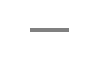
\begin{tikzpicture}  \draw[gray, ultra thick] (0,0) -- (0.5,0.0); \end{tikzpicture}). El perfil de densidad del agua está por fuera de la membrana (\textcolor{babyblueeyes}{azul} \begin{tikzpicture}  \draw[babyblueeyes, ultra thick] (0,0) -- (0.5,0); \end{tikzpicture}). En la interfase se localiza la densidad de grupos fosfato (\textcolor{orange}{naranja} 
\begin{tikzpicture}  \draw[orange, ultra thick] (0,0) -- (0.5,0); \end{tikzpicture}) y glicerol éster (\textcolor{darkgreen}{verde} \begin{tikzpicture}  \draw[darkgreen, ultra thick] (0,0) -- (0.5,0); \end{tikzpicture}). 

%%%%%%%%%%% Figura %%%%%%%%%%%%
\begin{figure}[t!]
%\vspace{0.5cm}
    \centering
	\includegraphics[width=0.8\linewidth, height=\textheight, keepaspectratio]{fig/02_dm/density_all.png} 
	\caption[Perfil de densidad de carga en las membranas lipídicas.]{Perfil de densidad de carga en las membranas lipídicas en función de la distancia \textit{z}. Las líneas más delgadas del sistema PCPG corresponden a las densidades de carga del POPG.}
      \index{density}
    \label{fig:densidad}
\end{figure}
%%%%%%%%%%%%%%%%%%%%%%% Fin %%%%%%%%%%%%%%%%%%%%%%%%

%%paper eze Chemistry and Physics of Lipids 213 (2018) 111–117
Una propiedad que se relaciona con la fluidez de la membrana es el \ac{apl}, a su vez esta propiedad está relacionada con el parámetro de orden de las colas hidrofóbicas del lípido, la compresibilidad y el empaquetamiento molecular \citep{Gapsys2013, Saeedimasine2019}. Además, el \ac{apl} también se puede emplear como un criterio para determinar si un sistema ha alcanzado el estado de equilibrio. La evolución del \ac{apl} en el tiempo se muestra en la \textbf{figura} \ref{fig:apl_zThick} (panel superior). Todos los sistemas alcanzan un estado de equilibrio desde los $\Xapprox$ 0.1 $\mu$s de simulación. \ac{dppc} presentó menor área promedio por lípido (68.8 \textpm 0.5 Å\textsuperscript{2}), valor que concuerda con lo reportado en literatura \citep{Petrache2000}. El sistema con mayor valor de \ac{apl} fue \ac{popg} con un promedio de 74.5 \textpm 0.5 Å\textsuperscript{2}, valor que concuerda con lo reportado en literatura \citep{Baoukina2012, Drabik2020, Kucerka2011, Shahane2019}. Respecto \ac{dppc}, es un lípido con un grupo polar más pequeño comparado al \ac{popg} que tiene un grupo polar con carga negativa, con un grupo polar más voluminoso y por tanto ocupa mayor área por molécula. En cuanto a los otros dos sistemas (\ac{popc} y PCPG), el \ac{apl} de PCPG es ligeramente mayor que \ac{popc} puro. 


La \textbf{figura} \ref{fig:apl_zThick} (panel inferior) muestra el espesor de la membrana (D$_{HH}$) para todos los sistemas simulados, este se determinó midiendo la distancia en \textit{z} entre los grupos fosfatos de la hemicapa superior e inferior \citep{Smith2021}. Los valores de D$_{HH}$  fueron similares con una mínima diferencia para \ac{dppc}. Además con este parámetro y el \ac{apl} se calculó el volumen por lípido, V$_{L} = \frac{APL\;x\;D_{HH}}{2}$. El orden del V$_{L}$ de mayor a menor fue: \ac{popg}>PCPG>\ac{popc}>\ac{dppc}. El V$_{L}$ es importante porque puede ser un indicativo para tener una idea del número de lípido que tienden a permanecer cerca del heterodímero $\alpha$IIb$\beta$3. Por lo tanto, es de esperarse que en el sistema  \ac{dppc} haya un mayor número de lípidos formando un anillo alrededor de los péptidos, mientras que para \ac{popg} deberían haber menos lípidos.
%%%%%%%%%%% Figura %%%%%%%%%%%%
\begin{figure}[t!]
    \centering
	\includegraphics[width=0.99\linewidth, height=\textheight, keepaspectratio]{fig/02_dm/ApL_zthickness_all.png} 
\caption[Área por lípido y espesor de membrana.]{Área por lípido y espesor de membrana.}
        \index{areaL}
    \label{fig:apl_zThick}
\end{figure}
%%%%%%%%%%%%%%%%%%%%%%% Fin %%%%%%%%%%%%%%%%%%%%%%%%

El parámetro de orden en modelo \ac{cg} (S$_{cc}$) para cada lípido se calculó con el programa \textit{LiPyphilic} \citep{Smith2021} empleando la ecuación \ref{ecu:scc},

\begin{equation}
S_{cc} = \frac{\langle 3 \cos^2 \theta \text{--}1 \rangle }{2}
\label{ecu:scc}
\end{equation}

donde el ángulo $\theta$ es el vector entre la normal a la membrana y el vector que conecta dos partículas \ac{cg} consecutivas. Los valores de \textit{S}$_{cc}$ para cada cadena hidrocarbonada se muestran en la \textbf{figura} \ref{fig:scc}. Los enlaces que están más próximos al grupo polar de los lípidos presentan mayor orden comparado a los enlaces de partículas en los extremos de la cadena hidrocarbonada. Además, se ve que todos los lípidos presentan un \textit{S}$_{cc}$ muy similar, excepto, la cadena ``sn1'' de \ac{dppc} que presenta valores ligeramente mayores indicando que la bicapa \ac{dppc} sería la membrana más compacta. Estos resultados concuerdan con lo observado anteriormente para \ac{apl} y V$_{L}$. La \textbf{tabla} \ref{tab:parame_lipid} resume estos párametros calculados.

%%%%%%%%%%% Figura %%%%%%%%%%%%
\begin{figure}[H]
    \centering
	\includegraphics[width=0.9\linewidth, height=0.9\textheight, keepaspectratio]{fig/02_dm/scc_all.png} 
\caption[Parámetro de orden de los lípidos]{Parámetro de orden de los lípidos. A) y B) hacen referencia a las cadenas hidrocarbonadas de cada lípido. Notar que C2A y C2B se resaltan en color diferente porque según el lípido de interés puede ser D2A y/o D2B. PCPG corresponde a la mezcla POPC:POPC 70\%:30\%.}
        \index{areaL}
    \label{fig:scc}
\end{figure}
%%%%%%%%%%%%%%%%%%%%%%% Fin %%%%%%%%%%%%%%%%%%%%%%%%

La \ac{rdf} se usó para identificar poblaciones de lípidos que se encuentran a una distancia menor a 20 \AA \,del heterodímero $\alpha$IIb$\beta$3 en plano \textit{xy}. La \textbf{figura} \ref{fig:rdf} muestra el perfil de las \ac{rdf}s de cada bicapa diferenciando entre hemicapa superior e inferior. Las distribuciones radiales de los lípidos en la hemicapa superior (\textbf{figura} \ref{fig:rdf}A) son ligeramente menores a las de la hemicapa inferior (\textbf{figura} \ref{fig:rdf}B) en el rango de 8 a 20 \AA \,. Esta diferencia incrementa a medida que los lípidos se encuentran lejos del heterodímero. En el rango de los 4 a 8 \AA \,,la bicapa de POPC presenta mayor densidad de lípidos cerca del heterodímero en la hemicapa inferior. Respecto a las otra bicapas, la distribución de lípidos es similar, aunque la RDF para los lípidos de POPG es ligeramente menor en ambas hemicapas. Los promedios de los parámetros de membrana anteriormente calculados se muestran en la \textbf{tabla} \ref{tab:parame_lipid}.

%%%https://gist.github.com/orbeckst/b611626e7640f399580e233195c6429c   cómo se calcula el RDF en MDAnalisys

%%%%%%%%%%% Figura %%%%%%%%%%%%
\begin{figure}[t!]
    \centering
	\includegraphics[width=0.8\linewidth, height=0.99\textheight, keepaspectratio]{fig/02_dm/rdfAll.png} 
	\caption[Función de distribución radial \textit{g(r)} para los lípidos respecto al heterodímero $\alpha$IIb$\beta$3.]{Función de distribución radial \textit{g(r)} para los lípidos respecto al centro de masa del segmento transmembrana del heterodímero $\alpha$IIb$\beta$3. A) y  B) corresponden a la hemicapa superior e inferior de la bicapa, respectivamente. La \textbf{figura} \ref{fig:rdf_allConverg} muestra el rango completo en la ordena \textit{x} de \textit{g(r)}.}
      \index{rdf}
    \label{fig:rdf}
\end{figure}
%%%%%%%%%%%%%%%%%%%%%%% Fin %%%%%%%%%%%%%%%%%%%%%%%%


%%%%%Tabla resumen membranas%%%%
\begin{table}[H]
  \begin{center}
%  \centering
  \caption[Resumen de los parámetros de membrana]{Resumen de los parámetros de membrana. Área molecular por lípido (APL), parámetro de orden  (S\textbf{\LARGE{$_{cc}$}}), espesor de membrana (D$_{HH}$) y volumen por lípido (V$_{L}$). El \ac{apl} y el D$_{HH}$ tienen un margen de error de \textpm 0.5 \AA\textsuperscript{2} y el S\textbf{\LARGE{$_{cc}$}} de \textpm 0.01.}
    \label{tab:parame_lipid}
  \begin{threeparttable}
 
    \begin{tabular}{l| c c c c}
      \toprule % <-- Toprule here
		Parámetro 					&  POPC	& POPG 	& PCPG 	& DPPC \\ 
      \midrule % <-- Midrule here
		APL (\AA\textsuperscript{2}) & 72.2 	& 74.5 	& 72.8 	& 68.8 \\ 

		S\textbf{\LARGE{$_{cc}$}} 					& 0.52 	& 0.53 	& 0.54	& 0.56 \\ 

		D$_{HH}$ (\AA) 					& 35.4 	& 35.6 	& 35.6 	& 36.3 \\
		V$_{L}$ (\AA\textsuperscript{3}) &1277.9 & 1326.1 & 1295.8 	& 1248.7  \\  
      \bottomrule % <-- Bottomrule here
    \end{tabular}
    \end{threeparttable}
  \end{center}
\end{table}
%%%%Fin tabla#%%%%%%%%%
\vspace{-0.5cm}

\section{Interacción lípido-péptido}

\begin{figure}[b!]
\vspace{0.5cm}
    \centering
	\includegraphics[width=0.99\linewidth, height=0.99\textheight, keepaspectratio]{fig/02_dm/lipid_pept_contac_all.png} 
	\caption[Contactos lípido-péptido durante la dinámica]{Contactos lípido-péptido durante la dinámica. A-B) Frecuencia de contactos lípido-péptido de $\alpha$IIb y $\beta$3 respectivamente. C) Secuencia del segmento TM del heterodímero $\alpha$IIb$\beta$3. Cada residuo en el eje \textit{x} incluye las frecuencias de las cuatro composiciones lipídicas estudiadas.}
      \index{lipid_resid_contact}
    \label{fig:lipid_pept_contac_all}
\end{figure}
%%%%%%%%%%%%%%%%%%%%%%% Fin %%%%%%%%%%%%%%%%%%%%%%%%

Con la función de distribución radial se identificaron poblaciones de lípidos alrededor del heterodímero $\alpha$IIb$\beta$3. Resulta importante identificar con qué residuos interaccionan los lípidos más cercanos. Se consideró como contacto a todas aquellas partículas (tipo BB) del heterodímero que estuvieran a una distancia $\leq$ 6.0 \AA \,de la partícula fosfato (PO4) de cada lípido, distancia usada ampliamente para considerar que existe un contacto \citep{Hedger2019, Corradi2018, Sica2021, Zhekova2023}.
La \textbf{figura} \ref{fig:lipid_pept_contac_all}A-B muestra la frecuencia normalizada de lípidos que permanecen a una distancia $\leq$ 6.0 \AA \,del heterodímero $\alpha$IIb$\beta$3 durantente toda la dinámica. Los residuos subrayados (\rule{0.5cm}{0.4pt}) en la \textbf{figura} \ref{fig:lipid_pept_contac_all}C  corresponden al segmento \ac{tm}, se resaltan algunos residuos en colores diferentes importantes para el análsis de contactos. Se observa mayor frecuencia de contactos lípido-$\alpha$IIb (\textbf{figura} \ref{fig:lipid_pept_contac_all}A) comparado con lípido-$\beta$3. Los residuos P$^{965}$, W$^{967}$, K$^{989}$,  F$^{992}$ y F$^{993}$ de $\alpha$IIb presentaron una ligera mayor frecuencia de contactos tuvieron con lípidos, particularmente preferencia por lípidos \ac{popc} (\begin{tikzpicture}
\filldraw[popc] (0,0) rectangle (0.5,0.2); 
\end{tikzpicture}).


Por otro lado, el péptido $\beta$3 interacciona con lípidos a través de los residuos I$^{693}$, V$^{695}$, K$^{716}$, T$^{720}$, y H$^{722}$. Sin embargo, la interacción se da principalmente con los lípidos \ac{popc} y la mezcla PCPG (\begin{tikzpicture} \filldraw[pcpg] (0,0) rectangle (0.5,0.2); 
\end{tikzpicture}), siendo casi nula la interacción con \ac{popg} (\begin{tikzpicture} \filldraw[popg] (0,0) rectangle (0.5,0.2); 
\end{tikzpicture}) y \ac{dppc} (\begin{tikzpicture} \filldraw[dppc] (0,0) rectangle (0.5,0.2); 
\end{tikzpicture}). Esto sugiere que la función de distribución radial descrita anteriormente para \ac{popg}  y \ac{dppc}  se localiza alrededor del péptido $\alpha$IIb. La \textbf{tabla} \ref{tab:lipid_pept_contac} resume el número de lípidos en contacto con cada péptido.

%%%%%Tabla lipid-contacts%%%%
\begin{table}[H]
\begin{center}
\centering
    \caption[Número de lípidos en contacto con los péptidos.]{Número de lípidos en contacto con los péptidos.}
    \label{tab:lipid_pept_contac}
    
  \begin{threeparttable}
	\begin{tabular}{@{}ccccc@{}}
\toprule
                                   & \textbf{POPC} & \textbf{POPG}   & \textbf{PCPG}   & \textbf{DPPC}  \\ \cmidrule(l){2-5} 
\multirow{-2}{*}{Péptido} &
  $\overline{x}$\textpm std &
  $\overline{x}$\textpm std &
  $\overline{x}$\textpm std &
  $\overline{x}$\textpm std \\ \midrule
{\color[HTML]{FE0000} $\alpha$IIb} & 19.8\textpm4.8 & 12.1\textpm4.5 & 16.9\textpm5.4 & 13.8\textpm5.3 \\ 
{\color[HTML]{3531FF} $\beta$3}    & 11.1\textpm3.9 & 1.4\textpm4.0  & 13.9\textpm5.4 & 0.9\textpm2.5  \\ \bottomrule
\end{tabular}
\end{threeparttable}
\end{center}
\end{table}
%%%%%FIN Tabla lipid-contacts%%%%
%\vspace{-0.5cm}

En la región interfacial \ac{tm}-\ac{ic} (\textbf{figura} \ref{fig:lipid_pept_contac_all}C) ambos péptidos presentan residuos cargados positivamente. La presencia de las lisinas K$^{989}$, K$^{994}$ en $\alpha$IIb y K$^{716}$ en $\beta$3 interaccionan con el grupo fosfato de los lípidos. Kim et al. identificaron que la interacción PO$_{4}^{\text{--}}$--K$^{716}$ interviene en el control del ángulo de cruce e inclinación del heterodímero TM-IC $\alpha$IIb$\beta$3 \citep{Kim2012}. Los autores también demostraron que una mutación de este residuo y otros, disrumpe el estado inactivo de la integrina. Contrario a esta posición, Zhu et al. sugieren que la mutación de la K$^{716}$ conduce a la activación de la integrina porque se disrumpen los puentes de hidrógeno entre la cadena lateral de la lisina y la cadena carbonada de $\alpha$IIb \citep{Zhu2009}. Los estudios por \ac{rmn} en micelas sugieren que los residuos K$^{716}$LLITIHD$^{723}$ en $\beta$3 y K$^{989}$VGFFKR$^{995}$ en $\alpha$IIb presentan interacciones péptido-péptido y  algunos residuos interaccionan con lípidos contribuyendo a la estabilidad del heterodímero. %%%integrinas_tesis%%% Además 
Además, $\alpha$IIb presenta el motivo G$^{991}$FFKR$^{995}$ altamente conservado en hélices $\alpha$ \ac{tm} y crucial en la dimerización \citep{Leung-Hagesteijn1994, OToole1994, Hughes1996}. %%2018_TESIS-Linking
En este motivo se observaron interacciones lípido-péptido en las cuatro membrana simuladas.
%Respecto a la región interfacial \ac{ec}-\ac{tm}, en estudios previos \citep{Lau2009, Yang2009} se reportó que el anillo aromático de los triptófanos W$^{967}$ y W$^{968}$


%%%paper de Samson 2021_ansell_occupancy
A partir de estos contactos lípido-péptido, podemos plantearnos qué tiempo permanecen en contacto estos lípidos con el péptido. La ocupancia de interacción es definida como la fracción de tiempo en la simulación donde la partícula fosfato permanece en contacto con una partícula de un residuo del heterodímero \citep{Ansell2021}. La \textbf{figura} \ref{fig:occupancy} muestra que \ac{popc} permanece más tiempo interaccionando con $\alpha$IIb comparado con $\beta$3. La ocupancia de la mezcla PCPG fue similar para los dos péptidos. Por último, \ac{popg} y \ac{dppc} interaccionan poco tiempo con ambos péptidos. Todos los valores fueron normalizados por el número total de lípidos.


%%%Figura en commun_result/lipid_protein_contact
%%%%%%%%%%% Figura %%%%%%%%%%%%
\begin{figure}[H]
    \centering
	\includegraphics[width=0.75\linewidth, height=0.3\textheight, keepaspectratio]{fig/02_dm/occupancy_all.png} 
	\caption[Ocupancia de los lípidos en contacto con cada péptido.]{Ocupancia de los lípidos en contacto con cada péptido.}
      \index{occupancy}
    \label{fig:occupancy}
\end{figure}
%%%%%%%%%%%%%%%%%%%%%%% Fin %%%%%%%%%%%%%%%%%%%%%%%%

\section{Orientación del heterodímero TM-IC $\alpha$IIb$\beta$3 en la bicapa lipídica}

La integrina $\alpha$IIb$\beta$3 en su estado inactivo se caracteriza por presentar una asociación con una configuración definida entre los segmentos TM. Datos obtenidos en bicelas por \ac{rmn} \citep{Lau2009} sugieren que en el heterodímero, los dos segmentos TM forman un ángulo de cruce de $\Xapprox$ 25\textdegree. En solución CD$_{3}$CN/H$_{2}$O este ángulo es de $\Xapprox$ 30\textdegree \,\citep{Yang2009}.\\
Para la asociación de hélices \ac{tm} se deben favorecer ciertas interacciones: \ac{vdw}, puentes de hidrógeno, iónicas, polares, lípido-lípido, lípido-proteína \citep{Fleming2001, Moore2008}. Algunos estudios sugieren que hay ciertos motivos (grupo de residuos) que son relevantes en el proceso de asociación hélice-hélice. Motivos que incluyen Pro, Asn, Asp, His, Gly, y SxxG, QxxS, se encuentran en algunas estructuras de proteínas  \ac{tm} que asocian hélices $\alpha$. Las 18 subunidades $\alpha$ de integrinas se caracterizan por presentar un motivo  \underline{X}xxxG, donde \underline{X} puede ser: S, A, G en su segmento \ac{tm}.
En este caso particular nos centramos en la $\alpha$IIb que presenta el motivo GxxxG \citep{Litvinov2019}, el cual desempeña una función importante en el proceso de asociación del heterodímero $\alpha$IIb$\beta$3, además de contribuir en el ángulo de cruce entre las dos hélices. Por lo tanto, es importante estudiar cuál es la función del ambiente lipídico en la asociación del heterodímero y la orientación de cada uno de los segmentos en la membrana. A modo de ilustración, la \textbf{figura} \ref{fig:tilt_angle_all}A muestra el ángulo $\tau$ que se forma entre la normal de la membrana y eje principal de la hélice $\alpha$. La  \textbf{figura} \ref{fig:tilt_angle_all}B ilustra el ángulo de cruce entre dos hélices \ac{tm}. En la \textbf{figura} \ref{fig:tilt_angle_all}C se muestra algunas capturas a diferentes tiempos donde se observa visualmente la variación de los ángulos. La \textbf{figura} \ref{fig:lipid_pept_contac_all}C resalta el motivo GxxxG en $\alpha$IIb que proporciona estabilidad al heterodímero. Experimentalmente, se ha demostrado que la G$^{972}$ interacciona con V$^{700}$ y M$^{701}$ en $\beta$3, la G$^{976}$ con I$^{704}$. Además, la G$^{708}$ interacciona con las L$^{979}$ y L$^{980}$ de $\alpha$IIb que contribuyen en el cierre del ángulo de cruce del heterodímero \citep{Lau2009, Yang2009}.

%%%Figura en tesis_main/03_Figures/tilt/popc
%%%%%%%%%%% Figura %%%%%%%%%%%%
\begin{figure}[H]
    \centering
	\includegraphics[width=0.9\linewidth, height=0.6\textheight, keepaspectratio]{fig/02_dm/tilt_angle_all.pdf} 
	\caption[Esquema inclinación del heterodímero $\alpha$IIb$\beta$3 respecto a la normal de la bicapa.]{Esquema inclinación del heterodímero $\alpha$IIb$\beta$3 respecto a la normal de la bicapa.}
      \index{tilt_angle_all}
    \label{fig:tilt_angle_all}
\end{figure}
%%%%%%%%%%%%%%%%%%%%%%% Fin %%%%%%%%%%%%%%%%%%%%%%%%

El ángulo promedio de cruce entre las dos hélices \ac{tm} fue $\Xapprox$ 33.5\textdegree \,en las cuatro membranas. Este resultado concuerda con los reportados experimentalmente \citep{Lau2009, Yang2009}. También por simulaciones \ac{dm} han reportado un valor promedio de 30\textdegree \,simulado en una bicapa de \ac{dppc} \citep{Kalli2011}. Experimentalmente no se ha determinado con precisión un valor del ángulo de inclinación, sin embargo, los valores estimados varían de 20\textdegree \, a 30\textdegree \, para $\beta$3 y 0\textdegree \, a 10\textdegree \,para $\alpha$IIb \citep{Lau2008, Lau2008a}. Por simulaciones se informaron valores de de 5\textdegree \, y 30\textdegree \,para $\alpha$IIb y $\beta$3, respectivamente \citep{Kalli2011}. En otro estudio Antreas Kalli obtuvo valores de $\alpha$IIb $\Xapprox$ 15\textdegree \,y $\beta$3 $\Xapprox$ 27\textdegree \,\citep{Kalli2013} por simulaciones de DM. El ángulo de inclinación de cada péptido es diferentes en las cuatro membranas lipídicas (\textbf{figura} \ref{fig:angles}).

%%%%%%%%%%% Figura %%%%%%%%%%%%
\begin{figure}[H]
    \centering
	\includegraphics[width=1\linewidth, height=0.99\textheight, keepaspectratio]{fig/02_dm/angles.png} 
	\caption[Distribución del ángulo de cruce del heterodímero $\alpha$IIb$\beta$3 y ángulos de inclinación de cada péptido respecto a la normal de la bicapa]{Distribución del ángulo de cruce del heterodímero $\alpha$IIb$\beta$3 y ángulos de inclinación de cada péptido respecto a la normal de la bicapa. Rojo y azul se corresponden a la distribución de ángulo de inclinación de $\alpha$IIb y $\beta$3, respectivamente. En verde la distribución del ángulo de cruce entre las hélices \ac{tm}.}
      \index{angles}
    \label{fig:angles}
\end{figure}
%%%%%%%%%%%%%%%%%%%%%%% Fin %%%%%%%%%%%%%%%%%%%%%%%%

%%%2018-TESIS
Un análisis más detallado de cada sistema se resume en los mapas de contactos entre los dos péptidos durante la dinámica, ver \textbf{figura} \ref{fig:contact_map}. El eje \textit{y} de cada mapa corresponde a los residuos del péptido $\alpha$IIb y el eje \textit{x} a $\beta$3. La escala a blanco (poca o nula interacción) y negro (alta interacción) representa los contactos entre determinados residuos. Al medio de los mapas de contacto se muestra parte de la estructura secundaria del $\alpha$IIb$\beta$3 y algunos residuos destacados para durante el análisis, esta representación corresponde a la secuencia que se muestra en la \textbf{figura} \ref{fig:contact_map}E. La diferencia más notable entre los cuatro sistemas se observa con \ac{dppc} (\textbf{figura} \ref{fig:contact_map}D). Varios contactos interaccionan menos tiempo en comparación a las otras membranas y también se observan contactos nuevos respecto a los otros sistemas. Por ejemplo, en la región interfacial EC-TM contactos como W$^{968}$--V$^{696}$, W$^{968}$--V$^{700}$, V$^{969}$--L$^{697}$, V$^{969}$--V$^{700}$ y V$^{969}$--A$^{703}$ interaccionan menos tiempo en DPPC. En esta misma región hay contactos de baja frecuencia (gris claro) que no vemos en los demás ambientes lipídicos: P$^{965}$--V$^{696}$, P$^{965}$--L$^{697}$, P$^{965}$--V$^{700}$, I$^{966}$--L$^{694}$ y I$^{966}$--L$^{697}$. Continuando en la diagonal del mapa de contactos del mismo sistema DPPC, el motivo GxxxG en $\alpha$IIb presenta contactos de baja frecuencia con residuos de $\beta$3 (\begin{tikzpicture}  \draw[deeppink, ultra thick, dotted] (0,0) -- (0.8,0.0); \end{tikzpicture}). En todos los sitemas se consevaron los contactos entre G$^{976}$--I$^{704}$ y L$^{980}$--G$^{708}$, mientras que los contactos que forma la G$^{972}$, G$^{976}$, L$^{979}$ con otros residuos de $\beta$3 disminuyeron en tiempo de interacción respecto a los otros sistemas. Además, hay nuevos contactos de baja frecuencia, por ejemplo: V$^{973}$--V$^{700}$, L$^{975}$--I$^{704}$, G$^{977}$--G$^{708}$, L$^{980}$--L$^{705}$. Se han realizado mutaciones del motivo GxxxG en $\alpha$IIb y de la G$^{708}$ en $\beta$3 \citep{Li2005, Luo2005}, concluyendo que cualquier mutación sobre este motivo disrumpe el ensamble de las hélices induciendo la activación de la integrina. Continuando hacia abajo en la diagonal, otros contactos con menor fecuencia de interacción durante la dinámica son: V$^{984}$--L$^{712}$, L$^{985}$--W$^{715}$ y M$^{987}$--L$^{712}$; éstos tres contactos son bien conservados en las otras tres bicapas. Más cerca a la región interfacial TM-IC los contactos M$^{987}$--I$^{719}$  (\begin{tikzpicture}  \draw[orange, ultra thick, dotted] (0,0) -- (0.8,0.0); \end{tikzpicture}) y G$^{991}$--I$^{719}$ son los únicos que se conservan en las bicapas excepto en DPPC que disminuye su frecuencia de interacción. Ésta región es la que mayor diferencia presenta en los cuatro sistemas. Observemos en DPPC (\textbf{figura} \ref{fig:contact_map}D, inferior derecha) el residuo I$^{719}$ en $\beta$3 además de interaccionar con M$^{987}$ y G$^{991}$, también interacciona con una frecuencia intermedia con F$^{993}$, similar a POPC sin embargo, este contacto es fuertemente marcado en las bicapas de POPG y PCPG.
Otro contacto ampliamente estudiado que es relevante en el proceso de activación de la intergina es el puente salino formado entre la R$^{995}$ en $\alpha$IIb y el D$^{723}$ en $\beta$3 (\begin{tikzpicture}  \draw[blue, ultra thick, dotted] (0,0) -- (0.8,0.0); \end{tikzpicture}) \citep{Yang2009, Lau2008a, Favier2018, Partridge2005}. En la membrana \ac{dppc}, ésta interacción presenta baja frecuencia respecto a los otros sistemas. Estas diferencias podrían explicar por qué las distribuciones de los ángulos de inclinación y cruce entre las hélices \ac{tm} (\textbf{figura} \ref{fig:tilt_angle_all}B) son dispersas y toman un rango de valores muy amplio en DPPC. 
En la mezcla lipídica PCPG (\textbf{figura} \ref{fig:contact_map}C) la presencia de un 30\% de \ac{popg} en la membrana de \ac{popc} fortalece el contacto del puente salino R$^{995}$--D$^{723}$ siendo así el ambiente lipídico en el que permanece más tiempo en interacción. Además, la H$^{722}$ de $\beta$3 fortaleció notablemente su interacción con K$^{994}$ y R$^{995}$ en $\alpha$IIb (\textbf{figura} \ref{fig:contact_map}C, recuadro pequeño en rojo). Por el contrario un contacto que se pierde por completo fue F$^{993}$--H$^{722}$ donde la frecuencia de interacción se da en el siguiente orden \ac{popg}>\ac{popc}>PCPG. Los contactos K$^{994}$--L$^{718}$ y K$^{994}$--I$^{719}$ son los que duran más tiempo interaccionando respecto a los demás sistemas. El contacto F$^{993}$--I$^{719}$ no se observa en la 

%%%%%%%Hoja horizontal %%%%%%%%%%%%%%%%%%%%%%%%
\begin{landscape}
%%%%%%%%%%% Figura %%%%%%%%%%%% 
\begin{figure}[b]
 \centering
	\includegraphics[width=1\linewidth, height=1.2\textheight, keepaspectratio]{fig/02_dm/contact_map.png}
	\caption[Mapa de contactos entre residuos del segmento \ac{tm}-\ac{ic} $\alpha$IIb y $\beta$3 en bicapas lipídicas]{Mapa de contactos entre residuos del segmento \ac{tm}-\ac{ic} $\alpha$IIb y $\beta$3 en bicapas lipídicas. E) Secuencia de residuos importantes en el análisis de contactos.}
        \index{contact_map}
    	\label{fig:contact_map}
\end{figure}
\end{landscape}
%%%%%%%%%%%%%%%%%%%%% Fin %%%%%%%%%%%%%%%%%%%%%%%

\noindent membrana POPG y presenta baja frecuencia en las membranas POPC y DPPC.
Las demás interacciones se conservan de forma similar a cuando los péptidos se encuentran en una bicapa pura de \ac{popc} o \ac{popg}.


Comparando los sistemas \ac{popc} y \ac{popg}, la mayoría de los contactos entre las hélices son similares, sin embargo, en la región próxima a la TM-IC algunos contactos son más estables en \ac{popg} respecto al \ac{popc}. La F$^{993}$ de subunidad $\alpha$IIb permanece más tiempo en contacto con la H$^{722}$ y la I$^{719}$ de $\beta$3 a su vez, la F$^{993}$ interacciona más tiempo con la L$^{718}$ en $\beta$3. El puente salino R$^{995}$ en $\alpha$IIb y el D$^{723}$ en $\beta$3, también permanece más tiempo en contacto en la membrana de \ac{popg}, además, estos residuos interaccionan más tiempo con otros residuos cuando se encuentran en la membrana con carga negativa. La R$^{995}$ interacciona con I$^{719}$ y T$^{720}$; el D$^{723}$ de $\beta$3, interacciona por un tiempo más prolongado con F$^{998}$ y F$^{999}$. Por último, en \ac{popg} los residuos K$^{725}$, E$^{726}$ y F$^{727}$ de $\beta$3 interaccionan con la secuencia N$^{996}$--RPPL--$^{1000}$. Este pequeño cúmulo o clúster de interacciones se observa levemente en los otros tres sistemas simulados. Observando la estructura secundaria de cada péptido (\textbf{figura} \ref{fig:tm_domain}A-B), la subunidad $\alpha$IIb no tiene estructura definida en el segmento \ac{ic}, por lo tanto, esta región presenta alta flexibilidad, confiriendo mayor grado de libertad a los residuos para explorar diferentes posiciones espaciales. 

La \textbf{figura} \ref{fig:distance_contacts_all} muestra la distribución de las distancias de enlace de algunas de las interacciones mencionadas anteriormente. La distancia de enlace R$^{995}$--D$^{723}$, en la bicapa de \ac{dppc} es donde presenta mayor heterogeneidad con tendencia a tomar valores mayores a 6.0 \AA. Por el contrario, las distancias más cortas se observan en la bicapa PCPG, ésto concuerda con lo observado en el mapa de contactos (\textbf{figura} \ref{fig:contact_map}C) en donde se muestra una prolongada interacción. Las distribuciones de las interacciones G$^{972}$--V$^{700}$ y G$^{972}$--A$^{700}$ y G$^{972}$--I$^{704}$ son relativamente similares en todas las membranas, excepto en DPPC que su distribución esta ligeramente sesgada a valores > \, 6.5 \AA.  

%%%%%%%%%%% Figura %%%%%%%%%%%%
\begin{figure}[H]
\vspace{0.5cm}
    \centering
	\includegraphics[width=0.9\linewidth, height=0.99\textheight, keepaspectratio]{fig/02_dm/distance_contacts_all.png} 
	\caption[Distribución de las distancias de enlace de algunas interacciones entre residuos del heterodímero \ac{tm}-\ac{ic} $\alpha$IIb$\beta$3.]{Distribución de las distancia de enlace de algunas interacciones entre residuos del heterodímero \ac{tm}-\ac{ic} $\alpha$IIb$\beta$3.}
      \index{distance_contacts_all}
    \label{fig:distance_contacts_all}
\end{figure}
%%%%%%%%%%%%%%%%%%%%%%% Fin %%%%%%%%%%%%%%%%%%%%%%%%


\section{Discusión del capítulo}

%%%%2017_Helix-helix
	Se han realizado varios estudios enfocados en la interacción hélice-hélice de la integrinas. Algunas de las técnicas experimentales empleadas son FRET y RMN en micelas de detergentes, bicelas y liposomas \citep{Mineev2014, Merzlyakov2006}. Estos estudios se enfocan principalmente en el efecto de la sustitución de residuos en la asociación de las hélices TM. Se encontró que en muchos casos las mutaciones causan la activación de la integrina, esto significa que disminuye la propensión a la formación del heterodímero de hélices $\alpha$ TM, aunque también se han observado mutaciones que inducen en estado inactivo de la integrina \citep{Lau2009}. Sin embargo, el efecto del ambiente lipídico no ha sido considerado en este proceso biológico. Por otra parte, varios estudios sugieren que las propiedades de los lípidos en la bicapa son importantes en la termodinámica de asociación y dimerización de proteínas de membrana. Por ejemplo, se ha observado que la fase gel de la membrana tiene un impacto favorable en la energía libre de la interacción hélice-hélice comparado a membranas con la fase líquido cristalino \citep{Anbazhagan2010}. Una razón por la cual se debe esta mejora de la dimerización en la fase gel más ordenada es el mayor costo energético de la incorporación de una hélice de proteína en ella, esto que hace que el estado dimérico con una superficie más pequeña sea más preferible.

	Hemos mencionado que el segmento \ac{tm} de $\alpha$IIb$\beta$3 es relevante para el proceso de activación de la integrina. En este capítulo se obtuvo información relevante acerca de cómo el ambiente lipídico regula la orientación del segmento \ac{tm} de $\alpha$IIb$\beta$3. Respecto a la \textbf{interacción lípido-péptido} el orden de interacción y ocupancia (porcentaje de tiempo que permanece en contacto) lípido-$\alpha$IIb fue POPC>PCPG>POPG>DPPC, mientras que lípido-$\beta$3 fue POPC>PCPG\(>\!\!>\)POPG>DPPC. En los dos péptidos la interacción con los lípidos se favorece más en la región interfacial TM-IC (hemicapa superior) comparado a la región interfacial TM-EC (hemicapa inferior). Esta diferencia de número de contactos lípido-péptido entre las hemicapas está influenciada por la flexibilidad de los segmentos IC de cada péptido que le permite a los residuos de la interfaz explorar diferentes posiciones en el espacio.	
	El grupo polar de los lípidos también influye en la asociación de hélices TM: lípidos aniónicos forman dímeros menos estables \citep{Hong2011}. Estas interacciones pueden verse de forma dualista: ya sea como la dimerización de la integrina $\alpha$IIb$\beta$3 que hace que la proteína adapte el entorno lipídico a sus preferencias, o como ciertos entornos lipídicos que favorecen la asociación de $\alpha$IIb$\beta$3. En rigor, estos puntos de vista son complementarios entre sí y ambos efectos se producen al mismo tiempo. La \textbf{figura} \ref{fig:rdf}B muestra la preferencia de lípido POPC y DPPC a localizarse más cerca al heterodímero comparado a la membrana de POPG.
		
	 Algunos de los residuos de $\alpha$IIb que interaccionan con lípidos son: W$^{967}$, K$^{989}$, V$^{990}$, F$^{992}$ y F$^{993}$; en $\beta$3 los contactos más relevantes fueron con los residuos: K$^{716}$, T$^{720}$ (ver \textbf{figura} \ref{fig:lipid_pept_contac_all}A-B). Éstos contactos lípido-péptido pueden influir en la conformación y orientación individual de cada péptido así como en la estabilidad segmento TM \citep{Stangl2015}. Además, el grupo de residuos K$^{989}$VGFFK$^{994}$ interacciona con lípidos y se ha reportado que contribuye en ángulo de cruce entre los dos segmentos TM \citep{Lau2008,Zhu2009}, por lo tanto, acá se podría alterar la estabilidad del heterodímero. Además, interacciones no específicas de lípidos también son comunes en las membranas biológicas. Por ejemplo, lípidos con cadenas de carbono insaturadas tienden a localizarse cerca de las hélices TM \citep{Flinner2015}. Esto va en el mismo sentido a lo observado con lípidos de POPC y DPPC cerca de los heterodímeros. POPC se ordena alrededor péptidos TM a través de la formación de una capa lipídica ordenada más grande, que es en muchos aspectos análogo al efecto hidrofóbico de las proteínas de membrana solubles en un ambiente acuoso \citep{Bocharov2017}. Interacciones electrostáticas se han estudiado entre la R$^{995}$ y lípidos como POPS y PIP2 \citep{Orowski2015, Schmidt2015}. En ambos estudios la interacción R$^{995}$-lípido disrumpen el puente salino entre R$^{995}$ en $\alpha$IIb y D$^{723}$ en $\beta$3.

	Las hélices TM tienen una orientación preferente relativa al plano de la membrana. Para cada péptido se calculó el de inclinación respecto a la normal de la membrana y el ángulo de cruce entre las dos hélices TM.  El motivo G$^{972}$xxxG$^{976}$ en $\alpha$IIb desempeña una función importante en la determinación de este ángulo entre las dos hélices TM y como mencionaremos más adelante, los contactos que forma este motivo con residuos de $\beta$3 no se vieron significativamente alterados, excepto en la membrana DPPC. Los ángulos de inclinación de cada péptido presentaron diferencias entre una membrana y otra, específicamente cuando se encuentra en un ambiente de DPPC. Incluso en DPPC el ángulo de cruce explora posiciones con ángulos de inclinación menores a 30\textdegree \,y mayores a 40\textdegree . Con base en estos resultados vemos cómo la inclinación de los péptidos es modifica según la composición de la membrana. 
Experimentalmente se ha reportado que el ángulo de inclinación de $\beta$3 se mantiene oscilando entre 25\textdegree \,y 30\textdegree \,. En esta orientación la cadena lateral con carga positiva de la K$^{716}$  interacciona con el grupo polar negativo del fosfato cerca de la interfaz membrana-agua \citep{Lagarrigue2016}. Un cambio en el ángulo de inclinación causada por la pérdida de la orientación de la K$^{716}$ puede disrumpir el heterodímero $\alpha$IIb$\beta$3 e inducir la activación de la integrina. 

	%%%2015_Orlowski
	Por lo general, el segmento TM de las integrinas presenta dos regiones de interacción que estabilizan la conformación inactiva del heterodímero. Una de ellas es la que se establece entre el motivo altamente conservado G$^{991}$FFKR$^{995}$ de $\alpha$IIb y los residuos hidrofóbicos W$^{715}$ e I$^{719}$ de $\beta$3, siendo estabilizada por el puente salino R$^{995}$--D$^{723}$. Estas interacciones se conocen como cierre de la membrana interna (CMI). En el extremo opuesto de la membrana (hemicapa superior), la interacción entre G$^{708}$ de $\beta$3 y el motivo G$^{972}$xxxG$^{976}$ en $\alpha$IIb se denomina cierre de la membrana externa (CME). Es crucial destacar que las mutaciones en los residuos de cualquiera de estos sitios de interacción (CMI y CME) resultan en interacciones perturbadas de las hélices TM, lo que puede llevar a una integrina constantemente activa \citep{Ye2014, Lau2009}.
	Del análisis del mapa de \textbf{contactos péptido-péptido} se obtuvo información relevante que permite comprender cómo se ven alterados y/o se forman contactos entre los segmentos TM del heterodímero $\alpha$IIb$\beta$3. La región CMI del heterodímero $\alpha$IIb$\beta$3 presentó la mayor alteración en contactos péptido-péptido en las cuatro composiciones lipídicas estudiadas. En particular resulta relevante la función del ambiente lipídico en la interacción tipo puente salino entre R$^{994}$ en $\alpha$IIb y  D$^{723}$ en $\beta$3. En la membrana que menos se favorece dicha interacción es DPPC y se fortalece en PCPG. En este sentido DPPC fue la membrana que más alteró contactos del péptido-péptido comparado a los otros tres sistemas. Los contactos que forma el motivo G$^{972}$xxxG$^{976}$ con algunos residuos de $\beta$3 se mantuvieron durante toda la simulación, excepto en la membrana DPPC que se vieron afectados, particularmente las interacciones G$^{972}$--V$^{700}$ y L$^{979}$--G$^{708}$, y esta diferencia respecto a los observado en las otras tres membranas va en el mismo sentido de lo observado con las diferencias en las distribuciones de los ángulos de inclinación de cada péptido. Por lo tanto, podemos decir que el DPPC altera notablemente interacciones péptido-péptido, sin embargo, éstas modificaciones no logran la separación del heterodímero. 
\chapter{Conclusiones generales}

	Previo a esta tesis, los estudios de integrinas había sido enfocado principalmente al mecanismo de activación con énfasis en los aspectos estructurales de los segmentos EC, TM e IC, además en la identificación de ligandos (interacción ligando-proteína) y residuos claves en el mecanismo de activación. Con esto en mente hemos abordado el estudio de los segmentos TM e IC de la integrina $\alpha$IIb$\beta$3 desde una perspectiva poco explorada. En la presente tesis se estudió la función del \textit{ambiente lipídico} en la conformación del segmentos TM-IC del heterodímero $\alpha$IIb$\beta$3. El estudio  inició con la expresión y purificación de los segmentos TM-IC de $\alpha$IIb y $\beta$3. Se realizó una caracterización de las propiedades fisicoquímicas de las secuencias para cada péptido. Posteriormente se realizaron experimentos en monocapas de Langmuir para evaluar la actividad y orientación de cada péptido en monocapas de diferente composición lipídica en donde se evaluaron los siguientes parámetros de los péptidos puros y mezclas lípido-péptido:

      \begin{itemize}
        \item{actividad superficial $\pi$-A}
        \item{potencial de superficie}
        \item{momento dipolar}
        \item{módulo de compresibilidad}
        \item{miscibilidad lípido-péptido}
      \end{itemize}
      
    Por último, se realizaron simulaciones de dinámica molecular a nivel de \acf{cg}. Se construyeron sistemas de bicapas lipídicas (cuatro composiciones diferentes)  + los segmentos TM-IC del heterodímero $\alpha$IIb$\beta$3. Desde esta perspectiva se analizaron interacciones lípido-péptido, péptido-péptido. Además, se obtuvo información del efecto del ambiente lipídico en la conformación de $\alpha$IIb$\beta$3.
    
    Los resultados de área molecular media descritos en el \textbf{capítulo} \textbf{\ref{chap:mono}} sugieren que los péptidos presentan una orientación vertical respecto al plano de las monocapas de Langmuir. Además, hemos propuesto que en ésta orientación vertical el segmento IC está en contacto con la subfase acuosa y el domino TM queda expuesto hacia el aire.\\
  La elasticidad lateral de los lípidos se ve modificada por la presencia de los péptidos y el efecto depende de la fase de estado particular de cada lípido. Por ejemplo, ambos péptidos $\alpha$IIb y $\beta$3 disminuyen levemente el módulo de compresibilidad del POPC respecto al POPC puro. Por otra parte, el módulo de compresibilidad del DPPC es considerablemente reducido en las mezclas lípido-péptido respecto al DPPC puro. Este efecto incrementa con el aumento de la fracción de péptido. Es decir, los péptidos afectan levemente la elasticidad lateral de lípidos POPC que presentan fase LE, mientras en DPPC (fase LC), la elasticidad lateral es significativamente reducida. Esto indicaría que DPPC adquiere una fase menos ordenada que la LC debido a la presencia de los péptidos.
  El análisis de la miscibilidad de componentes indicó que ambos péptidos presentan interacciones repulsivas con el lípido DPPC, siendo este efecto más marcado con el péptido $\beta$3. Con las otras dos interfases lipídicas POPC y PCPG se dan interacciones atractivas lípido-péptido. La mezcla PCPG es la interfase que más interactúa atractivamente con los péptidos, particularmente con  $\beta$3 y éste comportamiento se fortalece con el incremento de la fracción de péptido en la monocapa.\\
  
  Finalmente en el \textbf{capítulo} \textbf{\ref{chap:dm}} mencionamos sobre la preferencia por ciertos lípidos en la interacción con los péptidos, indicando que la composición lipídica puede modular las interacciones y la conformación de los segmentos TM.
  
  Se identifican residuos específicos en los péptidos $\alpha$IIb y $\beta$3 que son relevantes en las interacciones con los lípidos, lo que sugiere sitios clave para la regulación de la conformación y estabilidad del heterodímero.
  
  Se evidencia que el ambiente lipídico modula las interacciones entre los segmentos TM del heterodímero, siendo particularmente relevante en la región TM-IC. También afecta los ángulos de inclinación de los péptidos. 
    
   Se destaca que la membrana DPPC tiene un efecto notable en las interacciones péptido-péptido y en los ángulos de inclinación de los péptidos.
    
    En resumen, las dinámicas proporcionan una comprensión detallada de cómo el ambiente lipídico puede regular la conformación y estabilidad del segmento TM de $\alpha$IIb$\beta$3, así como las interacciones entre los péptidos involucrados, lo que puede tener implicaciones importantes en la función de la integrina y en procesos biológicos relacionados.
\chapter{Limitaciones de los modelos y perspectivas}


\subsection{Limitaciones de los modelos}

Las membrana biológica de cualquier célula es un sistema altamente complejo al presentar diversos componentes como proteínas, lípidos y carbohidratos principalmente. Y la diversidad de cada uno de los componentes es amplia, es por esto que aislarlas en su contexto nativo no una tarea simple. Por esta razón surgen modelos que simplificados que permiten estudiar ciertos componentes aislados, como los empleados en esta tesis, las capas monomoleculares con sus ventajas mencionadas previamente en la \textbf{sección} \textbf{\ref{monocapas}} y las bicapas lipídicas. Aquí también es necesario mencionar que estos sistemas no representan la realidad de la dinámica los procesos biológicos de la membrana. Algunas de sus limitaciones son: 

\begin{itemize}
\item{Variedad de especies lipídicas: Las membranas biológicas contienen una gran variedad de especies lipídicas, mientras que los modelos artificiales suelen utilizar un número más limitado de lípidos.}

\item{Asimetría de los lípidos: Es difícil imitar la asimetría característica de la distribución de los lípidos en las bicapas de las membranas biológicas.}

\item{Otros componentes: Los modelos de membrana lipídica no tienen en cuenta otros componentes importantes de las membranas biológicas, como las proteínas y los elementos del citoesqueleto, que regulan la difusión de lípidos y proteínas a través de la membrana.}
\end{itemize}

El modelo CG Martini implica un grado de aproximación que surge de la pérdida de detalles atómicos y es probable que los valores de las propiedades e interacciones lípido-péptido y proteína-proteína estimadas presenten una desviación respecto a los valores medidos experimentalmente. En particular, algunos cambios locales en la estructura secundaria podría inducirse tras la unión de lípidos reguladores. Las restricciones diédricas de la columna vertebral de proteína estándar empleadas dentro del modelo Martini \citep{Risselada2009, Marrink2007} y la falta de direccionalidad del enlace de hidrógeno que surge del sistema de CG significa que los posibles cambios conformacionales inducidos por los lípidos no se capturan en los cálculos actuales. El modelo de agua polarizable \citep{Yesylevskyy2010} mejora la precisión de los cálculos de energía libre para dividir las cadenas laterales de aminoácidos en ambientes hidrofóbicos. Sin embargo, sigue habiendo una comprensión incompleta de su influencia en las interacciones lípido-agua y proteína-agua.


Estas limitaciones hacen que los modelos de membrana lipídica artificial no puedan reproducir completamente la complejidad y el funcionamiento de las membranas biológicas. Sin embargo, siguen siendo herramientas valiosas para el estudio de ciertos aspectos de la estructura y la dinámica de las membranas celulares.


\subsection{Perspectivas}

Experimentalmente sería conveniente realizar una optimización a la metodología de expresión y repurificación por HPCL. Para la expresión se puede aumentar la cantidad en masa de proteína fusión realizando cultivos en un bioreactor. Cambiar el medio de cultivo por ejemplo, un LB fortificado con nutrientes. La repurificación por HPLC se podría escalar a una columna semi-preparativa, de esta forma cargar mayor cantidad de péptido previo a la elución evitando la sobresaturación de la columna como sucede al usar una columna analítica.

Contando con una cantidad considerable de los péptidos entre 5 a 10 mg son varios los análisis biofísicos que se pueden realizar. Realizar experimentos de monocapas en el \ac{bam} para analizar la partición de los péptidos a determinadas fase lipídicas. Con la espectroscopia de absorción por reflexión infrarroja 
espectroscopía infrarroja de reflexión-absorción por modulación de la polarización (PM-IRRAS) se puede conocer en detalle la orientación de los péptidos en las monocapas \citep{Rabe2014}. La espectroscopia de dicroísmo circular de radiación orientada es otra técnica que se puede emplear para saber la orientación y conformación de los péptidos en \acf{mlvs} \citep{Muruganandam2013}.

Al inicio del desarrollo de esta tesis estuvimos realizando experimentos de micro calorimetría de barrido diferencial de los péptidos puros y mezcla lípido-péptido en \acf{mlvs} , sin embargo, por la limitada disposición de péptido puro no se continuaron. La finalidad de estas mediciones apuntaban a responder la pregunta cuál es la preferencia de partición de los péptidos en la fase gel o líquido cristalino de una membrana. También se realizaron mediciones preliminares por FTIR de los péptidos en MLV's enfocados a conocer el efecto de los lípidos sobre estructura secundaria.

Realizar simulaciones multiescala grueso y átomo integrado para obtener los perfiles de energía libre de las interacciones lípido-péptido \citep{Corey2019, Domanski2017, Hedger2016}. En primera instancia se realizarían simulaciones CG que permiten obtener una adecuada exploración de la interacción lípido-proteína e identificar los sitios de contacto, posteriormente convertir a modelo atomístico y correr simulaciones de átomo integrado para cuantificar las interacciones. Además, en el análisis de contactos lípido-péptido considerar diferentes partículas del lípido, es decir, incluir las colas hidrocarbonadas que también podrían interaccionar con los péptidos.

En humanos la membrana plasmática de eritrocitos tiene la composición lipídica en peso que se muestra  abajo \citep{Hildebrand1975, Bruce2002}. Realizar simulaciones de DM en un sistema más realístico en composición de la membrana podría aportar información más acertada sobre el efecto de la membrana en la conformación y orientación de la integrina.

%%%Thomas E. Andreoli et al., Membrane Physiology (1987), Table 1, Chapeter 27
\begin{table}[H]
\centering
%\caption{}
%\label{tab:my-table}
\begin{tabular}{ll}
\rowcolor[HTML]{EFEFEF}
\hline
Lípido                & \%   \\ \hline
colesterol            & 26.0 \\
fosfatidilcolina      & 17.5 \\
esfingomielina        & 16.0 \\
fosfatidiletanolamina & 16.6 \\
fosfatidilserina      & 7.9  \\
fosfatidilinositol    & 1.2  \\
otros                 & 12.5 \\ \hline
\end{tabular}
\end{table}

En el presente estudio se trabajó solo con los segmentos TM-IC, dado que ya se dispone de la estructura completa integrina $\alpha$IIb$\beta$3 \citep{Adair2023}. A nivel experimental también se podría contactar a los autores si acceden a compartir el plásmido de la estructura y abordar estudios biofísicos experimentales y por simulaciones de DM para responder la pregunta del efecto del ambiente lipídico en la conformación de la integrina completa.
%%
\begin{appendix}

%%%%%%%%%%%%%%%%%%%%%%%%%%%
\chapter{Estructura y nomenclatura de aminoácidos. Histéresis en monocapas. Función de distribución radial}
%%%%%%%%%%%%%%%%%%%%%%%%%%%

%%%%%%%%%%% Figura %%%%%%%%%%%%
\begin{figure}[H]
    \centering
	\includegraphics[width=1\linewidth, height=0.6\textheight, keepaspectratio]{fig/04_anexos/aminioA_CG.png} 
\caption[Estructura y nomenclatura de aminoácidos]{Estructura y nomenclatura de aminoácidos. Representación en modelo Martini CG. Figura adaptada de CC BY-SA 3.0 \url{https://commons.wikimedia.org/wiki/File:Amino_Acids.svg}.}
        \index{tabla_aa}
    \label{tab:tabla_aa}
\end{figure}
%%%%%%%%%%%%%%%%%%%%%%% Fin %%%%%%%%%%%%%%%%%%%%%%%% 

 %%%%%%%Hoja horizontal %%%%%%%%%%%%%%%%%%%%%%%%
\begin{landscape}
%%%%%%%%%%% Figura %%%%%%%%%%%%
\begin{figure}[h]
 \centering
	\includegraphics[width=1\linewidth, height=1.2\textheight, keepaspectratio]{fig/04_anexos/histeresisAll.png}
	\caption[Histéresis de los péptidos puros y mezclas lípido-péptido]{Histéresis de los péptidos puros y mezclas lípido-péptido.}
        \index{histeresisAll}
    	\label{fig:histeresisAll}
\end{figure}
\end{landscape}
%%%%%%%%%%%%%%%%%%%%% Fin %%%%%%%%%%%%%%%%%%%%%%%


%%%%%%%%%%% Figura %%%%%%%%%%%%
\begin{figure}[h]
 \centering
	\includegraphics[width=1\linewidth, height=1.2\textheight, keepaspectratio]{fig/04_anexos/rdf_allConverg.png}
	\caption[Convergencia de la función de distribución radial \textit{g(r)}]{Convergencia de la función de distribución radial \textit{g(r)}.}
        \index{rdf_allConverg}
    	\label{fig:rdf_allConverg}
\end{figure}

%%%%%%%%%%%%%%%%%%%%%%%%%%%%%%%%%%%%%%%
\chapter{Protocolo de expresión y purificación de péptidos $\alpha$IIb y $\beta$3}\label{Protocolo Plasmido}
%%%%%%%%%%%%%%%%%%%%%%%%%%%%%%%%%%%%%%%
\definecolor{ghostwhite}{rgb}{0.97, 0.97, 1.0}

\begin{center} % Center the TikZ picture
\begin{tikzpicture}

% Define box and box title style
\tikzstyle{mybox} = [draw=myblue, fill=ghostwhite, very thick,
    rectangle, rounded corners, inner sep=8pt, inner ysep=15pt]
\tikzstyle{fancytitle} =[fill=myblue!80, text=white]
\node [mybox] (box){%  
    \begin{minipage}{0.99\textwidth}
Las membranas biológicas son un ensamble complejo de una gran variedad de lípidos y proteínas que conjuntamente realizar procesos biológicos importantes a nivel celular. Con la finalidad de entender la funcionalidad de la membrana, resulta conveniente estudiar las proteínas que son intrínsecamente de membrana. La purificación de proteínas de membrana es un área considerablemente desafiante en la biología molecular \citep{Ma2013, Mathieu2019, Jeffery2016}. Un criterio esencial en la purificación de proteínas integrales de membrana es que la proteína debe ser removida cuidadosamente de su ambiente nativo (altamente hidrofóbico) y aislada individualmente en solución. Esto solo es posible realizando una secuencia de pasos específicos desde el momento de expresión o síntesis química, de tal forma que en cada paso se recupere la mayor cantidad de la proteína de interés hasta la solubilización con solventes. Si bien en la literatura se encuantran las intrucciones para la purificación de éstos péptidos \citep{Yang2009}, no fue sencillo replicar los resultados. En determinado momento después de varios meses de trabajo decidimos enviar la secuencia de los péptidos a una empresa extranjera para su producción por síntesis química y el resultado fue negativo luego de dos intentos, ambos péptidos precipitan en agregados insolubles. Por lo tanto, parte de esta tesis consistió en encontrar la condiciones de expresión y purificación que permitieran obtener una cantidad considerable (en masa) de cada péptido con alta pureza para realizar los experimentos. También hemos producido por expresión recombinante la proteasa \ac{tev} que normalmente se obtiene comercialmente a un alto costo. Particularmente en el grupo de investigación del Dr. Guillermo Montich fue la primera vez que se trabajó con proteínas transmembrana. De esta forma hemos dejado un protocolo detallado para la obtención de los segmentos \ac{tm}-\ac{ic} de $\alpha$IIb y $\beta$3, además, podría emplease para péptidos similares. \end{minipage}
};
\node[fancytitle, right=10pt] at (box.north west) {\Large{Purificación de proteínas transmembrana}};
\node[fancytitle, rounded corners] at (box.east) {\faComment };
\end{tikzpicture}%
\end{center}


\begin{table}[H]
  \begin{center}
  \centering
  \captionsetup{justification=centering}  % Center the caption
    \caption{Datos de proteína fusión, segmentos transmembrana, MBP y TEV.}
    \label{tab:dat_proteina}
    \begin{tabular}{l l| l l }
      \toprule % <-- Toprule here

		$\alpha$IIb-Fusión & 49.41 kDa 	& $\alpha$IIb 	& 6.05 kDa \\ 
		{\Large{$\varepsilon$}}$_{\alpha \text{IIb-Fusión}}$ & 85830 M$^{\text{-1}}$cm$^{\text{-1}}$ & {\Large{$\varepsilon$}}$_{\alpha \text{IIb}}$ & 16500 M$^{\text{-1}}$cm$^{\text{-1}}$ \\
		$\beta$3-Fusión 	& 52.11 kDa 	& $\beta$3 	& 8.76 kDa \\
		{\Large{$\varepsilon$}}$_{\beta \text{3-Fusión}}$ & 83310 M$^{\text{-1}}$cm$^{\text{-1}}$ & {\Large{$\varepsilon$}}$_{\beta \text{3}}$ & 13980 M$^{\text{-1}}$cm$^{\text{-1}}$ \\
      \midrule % <-- Midrule here
      MPB & 42.49 kDa 	& TEV 	& 28.62 kDa \\ 
      \bottomrule % <-- Bottomrule here
    \end{tabular}
  \end{center}
\end{table}

Los plásmidos pMAL-C2 que contienen la secuencia de los péptidos $\alpha$IIb y $\beta$3 fueron gentilmente donados por el Dr. Qin \citep{Yang2009}. 


\section{Transformación de bacterias \emph{E. coli} DH5$\alpha$}
      \begin{itemize}
      \item{Agregar 1-2 $\mu$L del plásmido a un eppendorf. Si se encuentra depositado en gota sobre papel, recortar una pequeña parte y cortar en pedazos pequeños}
        \item{Agregar 50 $\mu$L de buffer Tris 50 mM pH 8. Evitar diluir mucho}
        \item{Dejar 30 minutos en suspensión}
        \item{Rotular dos viales eppendorf según corresponda $\alpha$IIb ó $\beta$3 y conservar en frío.}
        \item{Agregar a cada vial 100 $\mu$L de la cepa \emph{E. coli} DH5$\alpha$}
        \item{Tomar 10 $\mu$L del plásmido resuspendido y transferirlos al vial que contiene la bacteria \emph{E. coli} DH5$\alpha$}
        \item{Tapar y dejar durante 30 minutos en frío. calentar baño termostático a 42\textdegree C}
        \item{Colocar los viales en el baño caliente durante 1 minuto y 30 segundos.}
        \item{Colocar en hielo por 5 minutos}
        \item{Agregar 900 $\mu$L de LB a los eppendorf anteriores ($\alpha$IIb y $\beta$3)}
        \item{Calentar a 37\textdegree C por 1 hora}
    \end{itemize}
        
\subsubsection{Cultivo en caja de Petri}

\begin{itemize}
\item{Utilizar 4 tubos, dos para $\alpha$IIb y dos para $\beta$3, en donde tendremos una siembra diluida y una concentrada, es decir, de los tubos eppendorf anteriores (900 $\mu$L de LB, 100 $\mu$L de la cepa E. coli DH5$\alpha$ y los 10 $\mu$L de la suspensión de cada plásmido = “células diluidas”). 
Centrifugar a 4000 rpm/5 min y descartar todo el sobrenadante ($\Xapprox$ 800 $\mu$L), a esto los llamaremos  = “células concentradas”. Resuspender en los $\Xapprox$ 200 $\mu$L que sobraron pipeteando lentamente y esa serán las “células concentradas”.}

\item{Rotular 4 cajas de Petri con medio LB (diluida y concentrada tanto para $\alpha$IIb como $\beta$3). Dispersar homogéneamente mediante a agitación con núcleos de ebullición de las células en el cultivo.} 

\item{Pipetear 100 $\mu$L de “células” y depositarlos sobre las perlitas, luego tapar la caja y agitar con la finalidad que se “depositen” células por todo el medio y obtener diferentes colonias de bacterias que se puedan aislar fácilmente}
\end{itemize}


\subsubsection{Aislamiento de colonias}
\begin{itemize}
\item{Identificar y aislar una colonia (usando un palillo) y sembrarla en una caja de Petri con el mismo medio (LB \textbf{con ampicilina 100 $\mu$g/mL}; previamente secar)}

\item{Además, los palillos que se usan en $\alpha$IIb$_{1,2}$ y $\beta$3$_{1,2}$ se introducen en los medios líquidos de LB en tubos de ensayo (2.5 mL LB con ampicilina \textbf{[100 $\mu$g/mL]}). La caja de Petri se incuba a 37 \textdegree C por más de 12 horas y los tubos de ensayo, con sus respectivas tapas se llevan a shaker a 37\textdegree C por más de 12 horas}

 \item{Guardar células en glicerol al 15\% a -80\textdegree C}
 
 \item{Para verificar la pureza y el masa molecular de cada plásmido realizar una extracción con kit comercial que disponga el laboratorio y seguir la indicaciones del proveedor.}

\end{itemize}

\textbf{Notas}:
\begin{itemize}
    \item{La idea de sembrar nuevamente en LB sólido es porque se obtienen colonias aisladas y una vez han crecido son las que se utilizan para extraer los plásmidos y sembrar nuevamente, pero en la cepa de expresión}
    
    \item{Los cultivos líquidos se hacen con la idea de que una vez se obtengan las células, se dejan en una solución de glicerol al 15\% a -80\textdegree C, y se usan como “solución stock” cuando se necesite obtener células con el plásmido para expresar}

    \item{Las cajas de los primeros 4 cultivos se guardan temporalmente en una nevera para tenerlas como respaldo}
    
   
    De cada tubo de ensayo de cultivo líquido de LB, se extraen 500 $\mu$L en un tubo eppendorf, previamente rotulado y agregar 500 $\mu$L de glicerol al 30\%, es decir se obtiene 1 mL de \textbf{solución stock de células} al 15\% de glicerol. Guardar cada tubo por duplicado a -80\textdegree C.

\end{itemize}


%%%%%%%%%%%%%%%%%%%%%%%%%%%%%%%%%%%%%%%
\section{Expresión, lisis y purificación de proteína fusión}\label{Protocolo_Fusion}
%%%%%%%%%%%%%%%%%%%%%%%%%%%%%%%%%%%%%%%

El siguiente protocolo se realizó para expresar 4 L de cultivo de \textbf{proteína fusión} a partir del \textbf{stock de células} de cada péptido.

\subsection{Expresión}

\subsubsection{Preinóculo en cepa \ac{ecoli} BL21(DE3)}
    \begin{itemize}
        \item{Agregar 100 $\mu$L de ampicilina stock [100 mg/mL] a un frasco de agar LB de 100 mL}
        \item{Agregar bacterias \emph{E. coli} DH5$\alpha$ transformadas. Usar punta amarilla}
        \item{Dejar overnight a 37\textdegree C con agitación constante}
\end{itemize}

\subsubsection{Crecer células e inducir con IPTG}

Para crecer las células se usar Erlenmeyers de capacidad y agregar 1 L de LB en cada uno suplementado con 1.0 mL de ampicilina [100 mg/mL].
    \begin{itemize}
        \item{Tomar 25 mL del precultivo y agregarlo a cada Erlenmeyer}
        \item{Crecer a 37\textdegree C con agitación constante hasta obtener una \ac{do} entre 0.7-0.8 ($\Xapprox$ 7 horas)}
        \item{Agregar 1.0 mL de IPTG 1 M [1.0 mM]$_{final}$ a cada Erlenmeyer}
        \item{Agregar de nuevo ampicilina, 500 $\mu$L a cada cultivo}
        \item{Dejar nuevamente a 37\textdegree C con agitación por 5 horas}
    \end{itemize}

\subsubsection{Centrifugar medios}
    \begin{itemize}
        \item{Trasvasar el cultivo a los frasco de polipropileno Nalgene (capacidad de 500 mL)}
        \item{Colectar células por centrifugación a 4\textdegree C, 4500 \ac{rpm} durante 30 minutos}
        \item{Descartar el sobrenadante}
    \end{itemize}

Después de obtener un \textbf{pellet} (precipitado) en cada frasco, juntar en 2 falcón de 50 mL y guardar a -20\textdegree C o a -80\textdegree C congelando previamente con nitrógeno líquido.

\subsection{Lisis de células}
Por geles \ac{sds} se vio que parte de la proteína fusión fue a cuerpos de inclusión, por lo tanto, para obtener la mayor cantidad de proteína se realizar la ruptura de las células por tres métodos de lisis: ciclos frío-calor, incubación con Lisozima-ADNasa, (Freeze/Thaw) y alta presión (homogeneizador Emulsiflex).

\subsubsection{Ciclos frío-calor}
     \begin{itemize}
         \item{Resuspender cada pellet en 25 mL buffer de lisis \ac{pbs} 20 mM, 300 mM NaCl y 20 mM imidazol} + Triton X-100 [0.25\%]$_{final}$ (v/v)
        \item{Congelar muestras con nitrógeno líquido y dejar a -80\textdegree C por 2 horas}
        \item{Descongelar en un baño de agua a temperatura ambiente}
        \item{Repetir proceso al menos 3 veces}
    \end{itemize}

\subsubsection{Incubación con Lisozima-ADNasa}
     \begin{itemize}
        \item{Agregar inhibidor de proteasa \ac{pmsf} a concentración [1 mM]$_{final}$}
        \item{Agregar lisozima bovina [5 mg/L cultivo]$_{final}$}
        \item{Agregar DNAsa [0.5 mg/L cultivo]$_{final}$}
        \item{Agregar EDTA [1.0 mM]$_{final}$}
        \item{Dejar a 4\textdegree C con agitación en rotor overnight}
    \end{itemize}

\subsubsection{Homogenizador Emulsiflex}
     \begin{itemize}
        \item{Pasar cada muestra al menos 4 veces por el Emulsiflex}
        \item{Fijarse visualmente en la densidad y flujo al salir del Emulsiflex}
        \item{Después de los 4 ciclos, la muestra debe ser casi un líquido fluido}
    \end{itemize}

Finalmente las muestras fueron centrifugadas a 9500 \ac{rpm} por 30 minutos a 4\textdegree C (Eppendorf Centrifuge 5804R), conservando el \textbf{sobrenadante}. 


\subsection{Purificación por \"{A}KTA}

\begin{itemize}
    \item{Elución}
     \begin{itemize}
        \item{Equilibrar la columna con buffer A (el mismo de lisis)}
        \item{Cargar el contenido de 2L de cultivo; si carga más podría sobre saturar la columna. Usar bomba peristáltica}
        \item{Lavar con 10 \ac{cv} pasando buffer A. NO DESCARTAR ya que por geles \ac{sds} se observó que había proteína fusión, por lo tanto, se pasó después nuevamente por la columna}
        \item{Llevar columna al \"{A}KTA y pasar otros 10-20 mL de buffer A para obtener una buena base de linea en el cromatograma}
        \item{Eluir con buffer B, gradiente de imidazol de 20 a 400 mM (\ac{pbs} 20 mM, NaCl 300 mM, 400 mM imizadol)}
        \item{Colectar fracciones}
    \end{itemize}
\end{itemize}

\subsection{Cambio de buffer de la proteína fusión}
Antes de cuantificar la concentración de cada proteína fusión, se procedió a concentrar todo el contenido de las fracciones colectadas en centricones Amicon Ultra-15 Centrifugal con 30 kDa de radio de corte y cambiar de buffer en columnas PD-10 Desalting (GE Healthcare).

     \begin{itemize}
        \item{Lavar centricones de \textit{cuttoff} 30 kDa con agua Milli-Q}
        \item{Juntar todas las fracciones colectadas}
        \item{Centrifugar a 4500 \ac{rpm} a 4\textdegree C por $\Xapprox$ 20 minutos. Conservar el contenido retenido}
        \item{Equilibrar columna con buffer C (\ac{pbs} 20 mM, NaCl 150 mM y 7.5\% glicerol (vol/vol) pH 7.4)}
        \item{Cargar muestra y eluir hasta casi sequedad}
        \item{Agregar buffer C, eluir}
        \item{Repetir hasta pasar toda la muestra previamente concentrada}
    		\item{Cuantificar por espectrofotometría \ac{uv}. Fraccionar \textit{cutoff} y guardar a -20\textdegree C/-80\textdegree C}
    		\item{}
    \end{itemize}
    
Detalles técnicos columnas PD-10 Desalting \url{https://www.scientificlabs.co.uk/handlers/libraryFiles.ashx?filename=Manuals_1_17085101_A.pdf}


\section{Clivar y dializar}\label{Protocolo_TEV}

Tener en cuenta que la relación \ac{tev}:proteína es 1:30 mol a mol, por lo tanto, calcular bien la cantidad proteasa a usar según las concentraciones de TEV--proteína.

    \begin{itemize}
        \item{Descongelar las muestras de proteína y agregar \ac{dtt} [1.0 mM]$_{final}$}
        \item{Agregar \textit{XX} $\mu$L de TEV a cada vial. Tapar y agitar suave}
        \item{Dejar a 30\textdegree C por al menos 48 horas}
        \item{Centrifugar todos los viales a 13 mil \ac{rpm} por 10 minutos a temperatura ambiente}
        \item{Recuperar el \textbf{sobrenadante}. Concentrar en Amicón Ultra-15 Centrifugal con 3 kDa de radio de corte a 4500 \ac{rpm} a 4\textdegree C por $\Xapprox$ 40 minutos }

        \item{Lavar las membranas con EDTA y bicarbonato de sodio a 60\textdegree C por 5 minutos. Pasar flujo de agua Milli-Q por la membrana o dejar en remojo con agitación suave por 2 horas}
        \item{Cerrar/sellar uno de los extremos de la membrana, verificar que este bien sellado}
        \item{Agregar la muestra evitando dejar aire pero lo suficiente para sellar el otro extremo. Colocar membranas en beaker de al menos 1 L con agua Milli-Q}
        \item{Dejar 4\textdegree C con agitación. Realizar dos cambios de agua al menos dos veces cada 8 horas}
        \item{Remover toda la muestra incluyendo el precipitado y pasarlo a un eppendorf. Centrifugar todos los viales a 13 mil \ac{rpm} por 10 minutos a temperatura ambiente}
        \item{Separar el \textbf{pellet}. Juntar los pellets en falcón de 50 mL y resuspender en buffer (fase móvil A (H$_{2}$O:\ac{acn} 60\%/\%40, vol/vol, \ac{tfa} 0.01\% vol/vol)}
        \item{Calentar a baño María $\Xapprox$ 40\textdegree C para facilitar la solubilización}
        \item{Fraccionar en eppendorf y centrifugar todos los viales a 13 mil \ac{rpm} por 20 minutos a temperatura ambiente}
        \item{Tomar sobrenadante, juntar nuevamente y filtrar con membranas PVDF 0.45 $\mu$m (Durapore Merck). Esto para proteger al máximo la columna del \ac{hplc}}   
\end{itemize}

%%%%%%%%%%%%%%%%%%%%%%%%%%%%%%%%%%%
\section{Repurificación de péptidos por HPLC}\label{Protocolo_HPLC}
%%%%%%%%%%%%%%%%%%%%%%%%%%%%%%%%%%%

Tenga presente que los solventes deben ser grado \ac{hplc}, el agua Milli-Q se debe filtrar con membranas PVDF 0.22 $\mu$m y desgasar. Se recomienda seguir los cuidados de la columna según el manual del usuario disponible en: \url{https://vneshbiotorg.ru/upload/welch/use-and-maintainance-of-hplc-column-welch%20materials.pdf}.

\subsection{Purgar equipo y equilibrar columna}
     \begin{itemize}
        \item{Lavar y purgar bombas y loop del \ac{hplc} con agua y luego con la fase móvil A}
        \item{Equilibrar columna. Fijarse si está en \ac{meoh} debe hacer el cambio con los cuidados necesarios de gradiente y flujo}
        \item{Correr al menos 10 \ac{cv} de fase móvil A a 1.0 mL/min a 40\textdegree C}
        \item{Verificar que la presión no sobrepase los 210 bar. Si los supera bajar el flujo}
    \end{itemize}

\subsection{Inyectar y correr muestra}
     \begin{itemize}
        \item{Cargar 1 mL en el loop de la muestra previamente solubilizada y filtrada}
        \item{Iniciar cromatografía con el gradiente especificado en la metodología}
        \item{Colectar todas las fracciones con señal en el \ac{uv} a 280 nm distinguiendo en los diferente picos cromatográficos, es decir, que se resuelvan bien en el tiempo. El pico de los péptidos corresponde al \ac{tr} de 40--45 minutos}
        \item{Equilibrar de nuevo y repetir proceso hasta pasar toda la muestra}
        \item{Lavar bien la columna y el equipo \ac{hplc}}
    \end{itemize}

\subsection{Liofilizar y remover TFA}
    Anteriormente se mencionó colectar las fracciones correspondientes a los picos del cromatograma que se resuelven bien entre ellos, esto para hacer seguimiento por geles \ac{sds}. El pico correspondiente a los péptidos puros sale a los 40 minutos.
     \begin{itemize}
        \item{Juntar todas las fracciones del minuto 40 en un balón de destilación y llevar a un rotaevaporador hasta sequedad}
        \item{Pasar balón a una línea de Schlenk o rampa de vacío con doble trampa de nitrógeno líquido
        \item{Realizar entre 3--4 lavados con \ac{acn}:H$_{2}$O:A. acético} al 60\%:20\%:20\% (vol/vol) para remover el \ac{tfa}}
        \item{Resuspender en \ac{acn}:H$_{2}$O 67\%:33\% (vol/vol) y verificar la presencia del \ac{tfa} a los 1671 cm$^{\text{--1}}$ por FTIR}
    \end{itemize}

\end{appendix}

\def\bibfont{\scriptsize} %%%reducir fontsize biblio
\addcontentsline{toc}{chapter}{Bibliografía}
\bibliographystyle{biblioStyle} %%%plainnat without doi, url, issn
\setlength{\parindent}{0pt} % Disable indentation within this group
\bibliography{biblio}



\includepdf[scale=1.03, page=-]{porta_cover/back.pdf}
\end{document}
